% Compilation instructions:
%   cd docs/
%   pdflatex pose_estimation_presentation.tex
%   (or compile from repo root with: TEXINPUTS=./docs: pdflatex docs/pose_estimation_presentation.tex)
%
% Video playback: Embedded videos require Adobe Acrobat Reader DC or compatible PDF viewer.
% Videos are embedded using media9 package and play on click (no autoplay).
%
% Template reused from: /Users/bishal/Library/CloudStorage/OneDrive-UniversityofMiami/PhD/PhD Talk/PhD Talk/scHiGex_slides.tex
\documentclass[serif, aspectratio=169, 9pt]{beamer}
\usepackage{pgfpages} % For notes display
\usepackage{svg}
\usepackage{multirow} % Put this in the preamble
\usepackage{caption} % Enables \captionof{table}
\usepackage[linesnumbered,ruled,vlined]{algorithm2e}

% Enable notes in a second window
% \setbeameroption{show notes on second screen=right}
  
\usepackage{ragged2e} % Add this to your preamble

\usepackage[T1]{fontenc} 
\usepackage{fourier} % see "http://faq.ktug.org/wiki/uploads/MathFonts.pdf" for
% other options
\usepackage[utf8]{inputenc}
\usepackage{hyperref}
% media9 must be loaded after hyperref
% Note: media9 requires specific PDF viewer support (Adobe Acrobat)
\usepackage{media9} % For embedded video playback
\usepackage{latexsym,amsmath,xcolor,multicol,booktabs,calligra}
\usepackage{graphicx,pstricks,listings,stackengine}
\usepackage{lipsum}
\usepackage{pgfpages}
\usepackage{subcaption}
\usepackage{amssymb}  % for \checkmark
\usepackage[most]{tcolorbox}
\usepackage{xcolor} % Required for color definitions
\usepackage{tikz}
\usetikzlibrary{shapes,arrows,positioning}

\definecolor{gold}{rgb}{1.0, 0.84, 0.0}

\tcbset{
  colback=gold!20,   % Background color
  colframe=black,    % Border color
  width=\textwidth,  % Box width
  sharp corners,     % No rounded corners
  boxrule=0.5mm,     % Border thickness
  top=1mm, bottom=1mm, % Vertical padding
  fontupper=\small    % Set font size inside the box
}

\author{\textbf{Bishal Shrestha}}
\title{Real-Time Object Pose Estimation\\on HSR in IsaacSim}
\date{\small Fall 2025}
% Note: Compile from docs/ directory, or set TEXINPUTS=./docs: before compiling
\usepackage{latexppt}

% defs
\definecolor{UM}{RGB}{0,80,48}
\def\cmd#1{\texttt{\color{UM}\footnotesize $\backslash$#1}}
\def\env#1{\texttt{\color{blue}\footnotesize #1}}
\definecolor{deepblue}{rgb}{0,0,0.5}
\definecolor{deepred}{RGB}{0,0,0}
\definecolor{deepgreen}{rgb}{0,0.5,0}
\definecolor{halfgray}{gray}{0.55}

\setbeamercolor{alerted text}{fg=UM}
% \setbeameroption{show notes on second screen=right}

\lstset{
basicstyle=\ttfamily\small,
keywordstyle=\bfseries\color{deepblue},
emphstyle=\ttfamily\color{UM},    % Custom highlighting style
stringstyle=\color{deepgreen},
numbers=left,
numberstyle=\small\color{halfgray},
rulesepcolor=\color{red!20!green!20!blue!20},
frame=shadowbox,
}    
   
\begin{document}

\begin{frame} 
    \begin{figure}[htpb]
        \begin{center}
            % TODO: Add UM logo if available: \includegraphics[keepaspectratio, scale=0.02]{figures/UM.png} 
        \end{center}
    \end{figure}
    \vspace*{-1cm}
    \titlepage
    \vspace*{-1.5cm}
    \begin{tikzpicture}[remember picture, overlay]
      \node[anchor=south east, xshift=-.2cm, yshift=0.5cm] at (current page.south east) {CSC752 Final Project};
  \end{tikzpicture}
\end{frame}  

\begin{frame}   
    \frametitle{Contents}
    % EXPLANATION: This slide provides navigation structure for the presentation, showing the four main sections: Problem & Background (motivation and fundamentals), System Design (architecture and algorithms), Results & Evaluation (quantitative metrics and visualizations), and Lessons & Conclusion (takeaways and final system characteristics).
    \begin{columns}
        \column{0.6\textwidth}
        \tableofcontents[sectionstyle=show,
        subsectionstyle=hide,
        subsubsectionstyle=hide]
        \column{0.4\textwidth}
        \centering
        \vspace{0.5cm}
        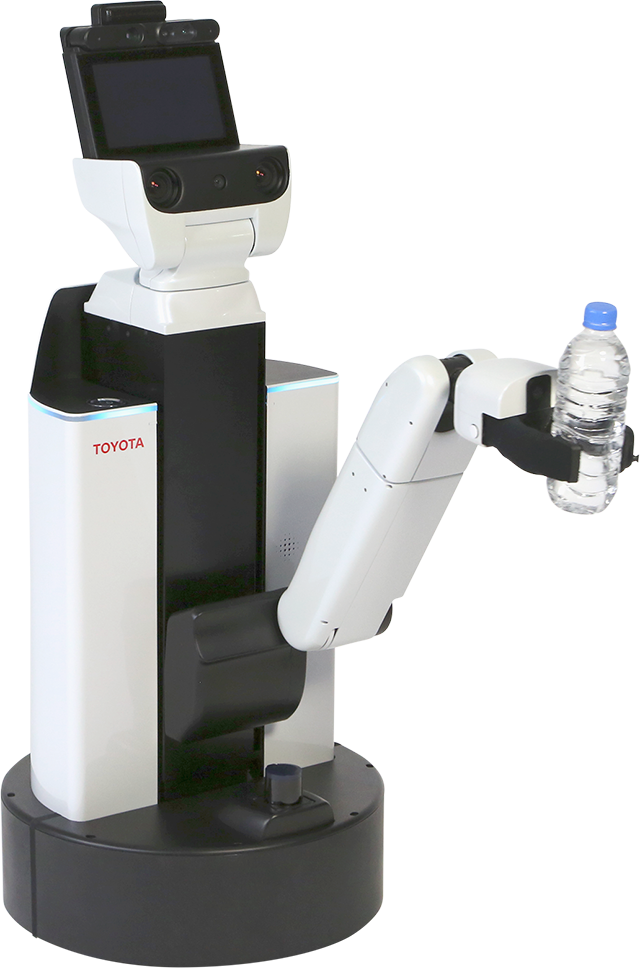
\includegraphics[width=0.9\linewidth,height=0.6\textheight,keepaspectratio]{../recordings/hsr2.png}
    \end{columns}
\end{frame}

% ============================================================================
% SECTION 1: Problem & Background
% ============================================================================

\section{Problem \& Background}

\begin{frame}
\frametitle{Problem \& Setup}
% EXPLANATION: This slide establishes the problem statement and system setup. It introduces the hardware platform (HSR robot in IsaacSim simulation), software stack (ROS1 in Docker for isolation), the goal (real-time 6D pose for manipulation), and inputs (RGB-D sensor data and object CAD models). The challenge emphasizes the need for accuracy, robustness, and speed simultaneously.
    \begin{columns}
        \column{0.48\textwidth}
        \begin{itemize}
            \item \textbf{Platform}: HSR robot + IsaacSim
            % EXPLANATION: HSR (Human Support Robot) is Toyota's mobile manipulator robot. IsaacSim is NVIDIA's physics-based simulation platform that provides realistic sensor data (RGB-D cameras) and robot dynamics. Using simulation allows safe testing and iteration before real-world deployment.
            \item \textbf{ROS1} inside Docker
            % EXPLANATION: ROS1 Noetic is the robotic operating system for inter-node communication. Docker containerization isolates the ROS1 environment, ensuring consistent dependencies and avoiding conflicts with system libraries (critical for cv_bridge and libffi compatibility).
            \item \textbf{Goal}: Real-time 6D pose for grasping
            % EXPLANATION: Real-world robotic manipulation requires the pose of the target object in the robot's base frame with minimal latency; 6D pose = 3D translation + SO(3) orientation. "Real-time" means pose updates fast enough for closed-loop control (typically < 1.5s total latency).
            \item \textbf{Input}: RGB-D from robot head, object meshes
            % EXPLANATION: RGB-D provides both color (photometric cues) and depth (geometric cues) from the robot's head-mounted camera. Object meshes (CAD models) are required by FoundationPose for pose estimation - the method aligns the observed RGB-D data with the known 3D geometry.
        \end{itemize}
        \vspace{0.3em}
        \begin{block}{Challenge}
            Accurate, robust, fast pose estimation for manipulation
            % EXPLANATION: These three requirements are often in tension: accuracy requires careful processing (slow), robustness needs redundancy/validation (slow), speed needs optimization (may sacrifice accuracy). The system must balance all three for successful manipulation - inaccurate poses cause grasp failures, non-robust systems fail under occlusion/lighting changes, slow systems can't support real-time control.
        \end{block}
        \column{0.5\textwidth}
        \begin{figure}
            \centering
            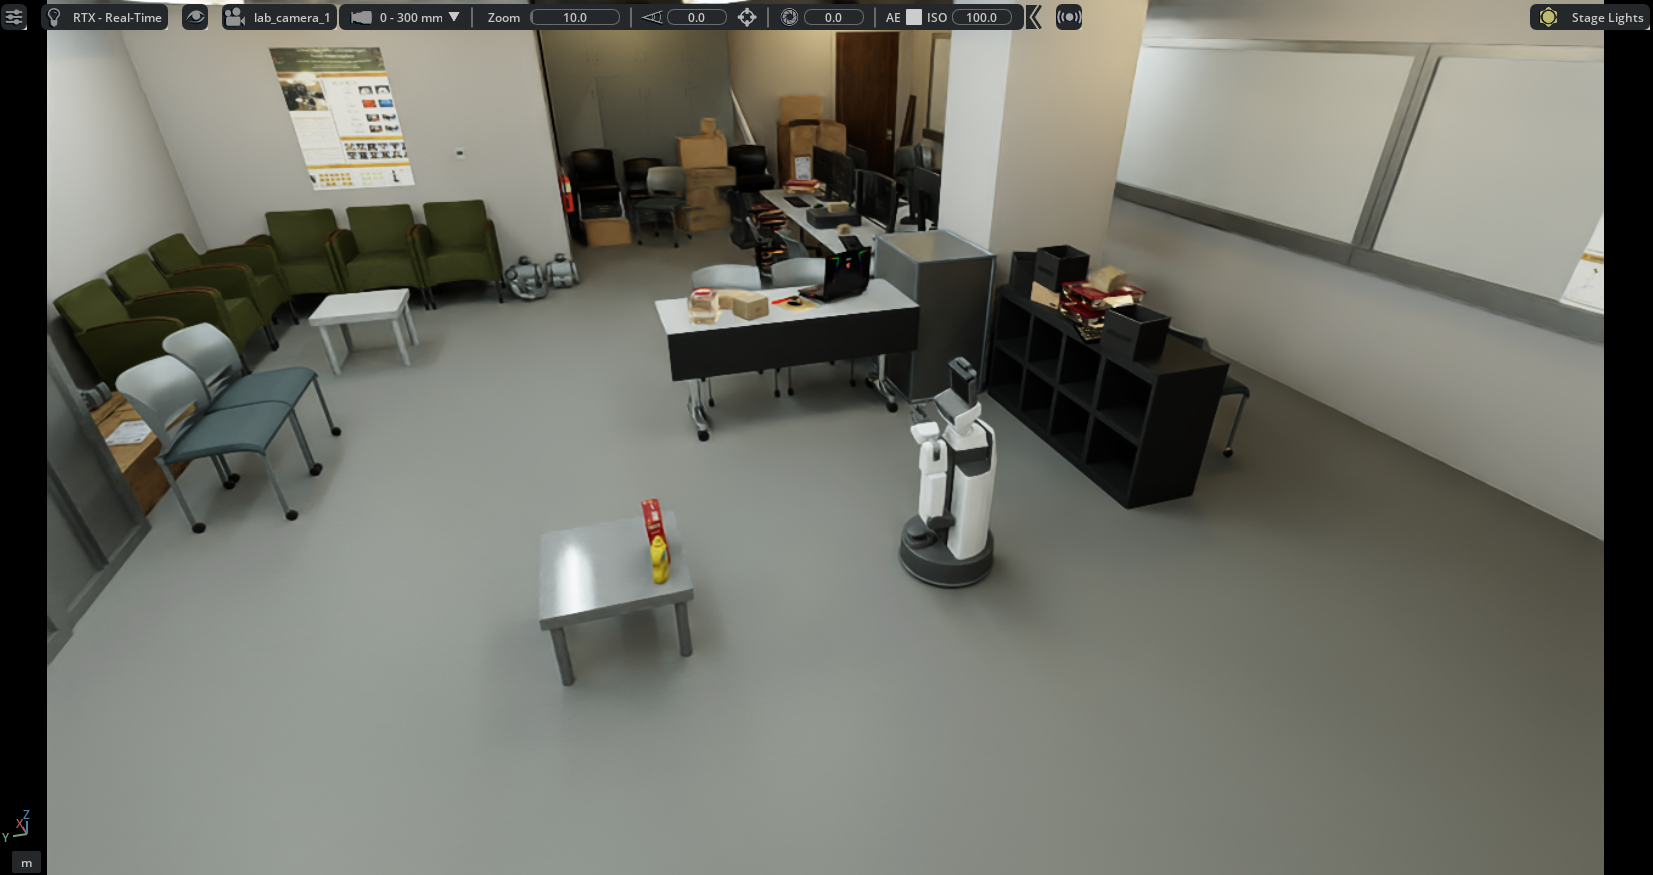
\includegraphics[width=1.05\linewidth,keepaspectratio]{../recordings/scene2.png}
            \caption{Simulation environment}
            % EXPLANATION: This image shows the IsaacSim simulation environment with the HSR robot, table, and objects. It demonstrates the realistic sensor simulation (lighting, shadows, physics) that enables testing pose estimation algorithms before real-world deployment.
        \end{figure}
    \end{columns}
\end{frame}

\begin{frame}
\frametitle{6D Pose Estimation Geometry}
% EXPLANATION: This slide explains the mathematical foundations of 6D pose estimation: coordinate frame transformations, pinhole camera projection model, and why RGB-D (depth) is essential. It establishes the geometric vocabulary needed to understand why segmentation quality matters (bad masks corrupt depth, leading to Z-axis errors).
    \begin{columns}
        \column{0.6\textwidth}
        \textbf{Coordinate Frames}
        \begin{itemize}
            \item \textbf{Object frame} $(O_o, X_o, Y_o, Z_o)$: Object-centered
            % EXPLANATION: The object frame is attached to the object itself, with origin at a canonical point (e.g., object center). This frame moves with the object. FoundationPose uses object-centric normalization to handle objects of different scales.
            \item \textbf{Camera frame} $(O_c, X_c, Y_c, Z_c)$: Camera-centered
            % EXPLANATION: The camera frame has origin at the camera's optical center, Z-axis along the viewing direction. RGB-D images are captured in this frame. The robot's TF tree transforms from camera frame to base frame.
            \item \textbf{6D pose}: $[R|t]$ transforms object $\to$ camera frame
            % EXPLANATION: The 6D pose is the rigid transformation (rotation matrix R in SO(3) + translation vector t in R^3) that maps points from object frame to camera frame. This is what FoundationPose estimates - where and how the object is oriented relative to the camera.
        \end{itemize}
        \vspace{0.3em}
        \textbf{Pinhole Projection}
        \begin{itemize}
            \item 3D point $P_o$ in object frame
            % EXPLANATION: A 3D point on the object's surface, expressed in object coordinates. FoundationPose uses dense correspondences (many points) rather than sparse keypoints.
            \item \textbf{Step 1 - Transform}: $P_c = R P_o + t$ (object frame $\to$ camera frame)
            % EXPLANATION: This rigid transformation converts coordinates from object's own coordinate system to camera's coordinate system. R (3x3 rotation matrix) rotates the point to match camera's orientation - if object is rotated 45°, R rotates the point by 45°. t (3D translation vector) shifts the point to camera's position - if object is 1m away, t moves the point by 1m. Together, R and t represent the 6D pose we're estimating: "where is the object relative to the camera?"
            \item \textbf{Step 2 - Project}: $p = K P_c / Z_c$ (3D camera frame $\to$ 2D image pixels)
            % EXPLANATION: This projects the 3D point onto the 2D image plane. First, K (intrinsic matrix) scales by focal length and shifts by principal point: $K P_c = [f_x X_c + c_x, f_y Y_c + c_y, Z_c]^T$. Then dividing by $Z_c$ (depth) implements perspective projection - objects farther away (larger $Z_c$) appear smaller. Result: $p = [u, v]^T$ is the 2D pixel coordinate where this 3D point appears in the image. This is why depth accuracy matters - wrong $Z_c$ leads to wrong pixel locations.
            \item $K = \begin{bmatrix} f_x & 0 & c_x \\ 0 & f_y & c_y \\ 0 & 0 & 1 \end{bmatrix}$: camera intrinsics matrix
            % EXPLANATION: K is a 3x3 matrix encoding camera's internal parameters: f_x, f_y are focal lengths (in pixels) for x and y axes, (c_x, c_y) is the principal point (image center, where optical axis intersects image plane). These parameters are obtained from camera_info topic via camera calibration. They're fixed for a given camera and must be accurate - errors in K cause systematic projection errors that corrupt pose estimation.
        \end{itemize}
        \vspace{0.3em}
        \textbf{RGB-D Advantage}
        \begin{itemize}
            \item Depth $Z_c$ directly measured
            % EXPLANATION: RGB-D sensors (like the HSR's head camera) directly measure depth at each pixel. This eliminates scale ambiguity present in monocular vision - we know absolute 3D positions, not just relative geometry.
            \item Resolves scale ambiguity
            % EXPLANATION: Monocular vision can only recover geometry up to scale (can't tell if object is small and close or large and far). Depth sensors provide absolute scale, enabling accurate 3D reconstruction and pose estimation.
            \item $Z_c$ most sensitive to mask errors
            % EXPLANATION: When segmentation mask leaks (includes table pixels), those pixels have wrong depth values (table is at different Z than object). FoundationPose uses depth for 3D reconstruction, so corrupted depth leads to corrupted 3D points, causing pose errors. Z-axis (height) is most affected because table and object are at different heights.
        \end{itemize}
        \column{0.38\textwidth}
        \begin{figure}
            \centering
            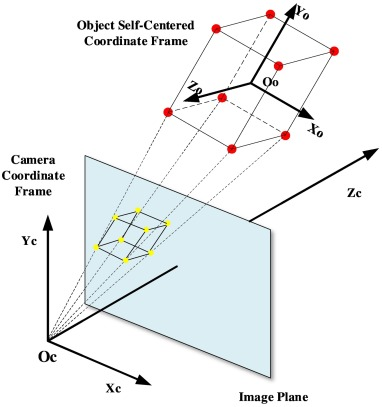
\includegraphics[width=\linewidth,height=4cm,keepaspectratio]{../recordings/pose_estimation.jpg}
            \caption{Real-time 6D pose estimation geometry from RGB-D image}
            % EXPLANATION: This diagram visualizes the coordinate frames (object frame O_o and camera frame O_c), projection rays from camera center through image plane, and how 3D object points project to 2D pixels. It shows why depth is needed - without Z_c, we can't determine where along the projection ray the 3D point lies.
        \end{figure}
    \end{columns}
\end{frame}

\begin{frame}
\frametitle{Mask Leakage (Segmentation Errors)}
% EXPLANATION: This slide explains mask leakage failure mode: when segmentation mask includes table pixels (leakage), those pixels have wrong depth values, corrupting 3D reconstruction and causing Z-axis instability. Shows how segmentation errors propagate to pose errors.
    \begin{columns}
        \column{0.48\textwidth}
        \textbf{Mask Leakage (Segmentation Errors)}
        \begin{itemize}
            \item Bad mask $\to$ corrupted depth
            % EXPLANATION: When segmentation mask includes table pixels (leakage), those pixels have depth values from the table surface (~0.6m) rather than the object (~0.8m). FoundationPose uses masked depth for 3D reconstruction, so wrong pixels lead to wrong 3D points.
            \item Depth noise $\to$ Z-axis instability
            % EXPLANATION: Corrupted depth values create inconsistent 3D points. When FoundationPose tries to align these points with the object mesh, the optimization becomes unstable. Z-axis (height) is most affected because table and object differ primarily in height.
            \item Height error: ~30cm drift
            % EXPLANATION: Measured error from monologue.md: without proper segmentation, height error was ~30cm (object height estimated incorrectly because table pixels pulled the estimate down). This is too large for precise manipulation.
        \end{itemize}
        \vspace{0.3em}
        \begin{block}{Key Insight}
            Segmentation quality $\to$ depth quality $\to$ pose stability
            % EXPLANATION: This is the core insight: segmentation quality directly determines which depth pixels are used. Good segmentation (clean mask) = good depth (only object pixels) = stable pose. Bad segmentation (leaky mask) = corrupted depth (table pixels included) = unstable pose with large errors.
        \end{block}
        \column{0.5\textwidth}
        \begin{figure}
            \centering
            \begin{subfigure}{0.48\textwidth}
                \centering
                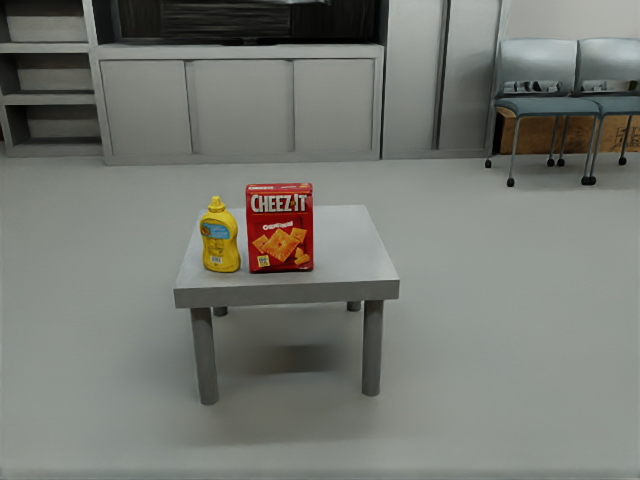
\includegraphics[width=\linewidth,keepaspectratio]{../debug/foundationpose/color.png}
                \caption{RGB image}
                % EXPLANATION: Original RGB image showing the object (mustard bottle) on the table. This is the input to segmentation.
            \end{subfigure}
            \hfill
            \begin{subfigure}{0.48\textwidth}
                \centering
                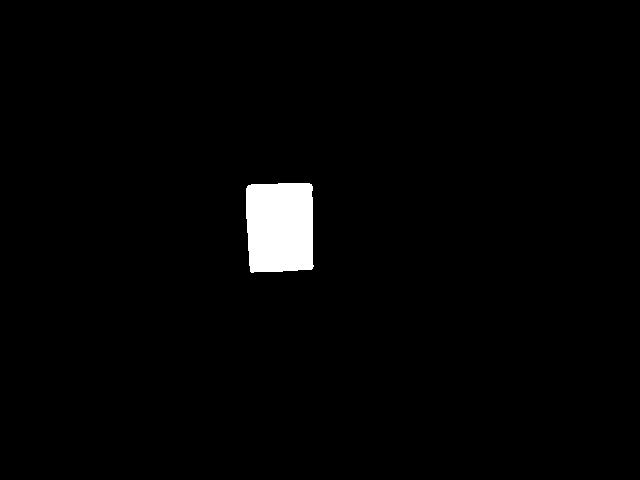
\includegraphics[width=\linewidth,keepaspectratio]{../debug/foundationpose/ob_mask.png}
                \caption{Object mask}
                % EXPLANATION: Segmentation mask from SAM showing object pixels (white) and background (black). This is a correct segmentation example. When mask leaks (includes table pixels around edges), those pixels have wrong depth values (~0.6m for table vs ~0.8m for object), corrupting 3D reconstruction and causing Z-axis instability (~30cm height error).
            \end{subfigure}
            \caption{Ideal scenario of RGB image and segmentation mask}
            % EXPLANATION: Left: RGB image showing object on table. Right: Segmentation mask from SAM showing object pixels (white) and background (black). This is a correct segmentation example. When mask leaks (includes table pixels around edges), those pixels have wrong depth values (~0.6m for table vs ~0.8m for object), corrupting 3D reconstruction and causing Z-axis instability (~30cm height error).
        \end{figure}
    \end{columns}
\end{frame}

\begin{frame}
\frametitle{Asynchronous Data (Timestamp Mismatches)}
% EXPLANATION: This slide explains asynchronous data failure mode: RGB, depth, and mask arrive at slightly different times. If robot is moving, using wrong timestamp for TF lookup gives wrong camera pose, causing pose jumps and temporal drift.
    \begin{center}
    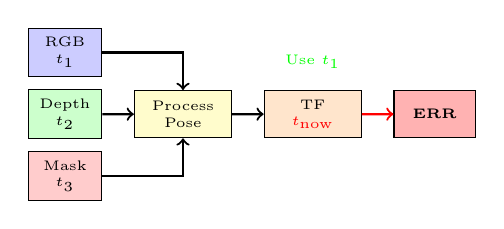
\begin{tikzpicture}[node distance=0.6cm, auto, font=\tiny, scale=0.8]
        % Messages arriving at different times (stacked vertically, then flow horizontally)
        \node[draw, rectangle, fill=blue!20, text width=0.7cm, text centered, minimum height=0.4cm] (rgb) {RGB\\$t_1$};
        \node[draw, rectangle, fill=green!20, text width=0.7cm, text centered, minimum height=0.4cm, below=0.15cm of rgb] (depth) {Depth\\$t_2$};
        \node[draw, rectangle, fill=red!20, text width=0.7cm, text centered, minimum height=0.4cm, below=0.15cm of depth] (mask) {Mask\\$t_3$};
        
        % Processing (centered vertically relative to the three inputs)
        \node[draw, rectangle, fill=yellow!20, text width=1cm, text centered, minimum height=0.6cm, right=0.4cm of depth] (process) {Process\\Pose};
        
        % TF lookup (wrong timestamp)
        \node[draw, rectangle, fill=orange!20, text width=1cm, text centered, minimum height=0.6cm, right=0.4cm of process] (tf) {TF\\\textcolor{red}{$t_{\text{now}}$}};
        
        % Error output
        \node[draw, rectangle, fill=red!30, text width=0.8cm, text centered, minimum height=0.6cm, right=0.4cm of tf] (error) {\textbf{ERR}};
        
        % Arrows from all inputs to process
        \draw[->, thick] (rgb) -| (process);
        \draw[->, thick] (depth) -- (process);
        \draw[->, thick] (mask) -| (process);
        
        % Arrows through pipeline
        \draw[->, thick] (process) -- (tf);
        \draw[->, thick, red] (tf) -- (error);
        
        % Annotation: should use t1
        \node[above=0.15cm of tf, font=\tiny] {\textcolor{green}{Use $t_1$}};
    \end{tikzpicture}
    \end{center}
    \vspace{0.3em}
    \begin{columns}
        \column{0.48\textwidth}
        \textbf{Asynchronous Data (Timestamp mismatches)}
        \begin{itemize}
            \item RGB, depth, mask arrive separately
            % EXPLANATION: ROS callbacks for RGB, depth, and mask topics fire independently. Even with TimeSynchronizer, there can be small timing differences. If robot is moving, camera pose changes between captures.
            \item Wrong TF lookup $\to$ incorrect $[R|t]$
            % EXPLANATION: TF transforms depend on time - robot pose changes as it moves. If we use TF lookup at wrong time (e.g., current time instead of image capture time), we get wrong camera-to-base transform, leading to wrong pose in base frame.
            \item Result: 3D pose jumps, temporal drift
            % EXPLANATION: Without timestamp sync, pose estimates jump around as TF lookups use wrong robot poses. Over time, errors accumulate causing drift. This was observed before implementing exact timestamp matching.
        \end{itemize}
        \column{0.5\textwidth}
        \begin{figure}
            \centering
            \begin{subfigure}{0.48\textwidth}
                \centering
                \textbf{T1}\\[0.2em]
                \includegraphics[width=\linewidth,height=3.5cm,keepaspectratio]{../frames.pdf}
                % EXPLANATION: Same figure shown at timepoint T1. Demonstrates how robot position and camera pose change over time, affecting TF transforms.
            \end{subfigure}
            \hfill
            \begin{subfigure}{0.48\textwidth}
                \centering
                \textbf{T2}\\[0.2em]
                \includegraphics[width=\linewidth,height=3.5cm,keepaspectratio]{../frames.pdf}
                % EXPLANATION: Same figure shown at timepoint T2. Shows how using wrong timestamp for TF lookup (e.g., T2 timestamp for T1 image) causes pose error. Robot has moved, so camera pose is different, leading to incorrect pose transformation.
            \end{subfigure}
            \caption{Timestamp mismatch causing pose drift}
            % EXPLANATION: Same figure at two different timepoints (T1 and T2). At T1, robot is at one position; at T2, robot has moved. If RGB/depth/mask arrive at slightly different times and we use wrong timestamp for TF lookup (e.g., T2 timestamp for T1 image), we get wrong camera-to-base transform, causing pose jumps and temporal drift. Demonstrates why exact timestamp matching is critical for moving robots.
        \end{figure}
    \end{columns}
\end{frame}

% \begin{frame}
% \frametitle{Noisy Boundaries (Refinement Instability)}
% % EXPLANATION: This slide explains noisy boundaries failure mode: when mask boundaries are noisy (pixels flicker in/out), FoundationPose's iterative optimization objective function changes between iterations, preventing convergence. Results in large position and orientation errors.
%     \begin{columns}
%         \column{0.48\textwidth}
%         \textbf{Noisy Boundaries (Refinement instability)}
%         \begin{itemize}
%             \item Unstable refinement iterations
%             % EXPLANATION: FoundationPose uses iterative optimization to refine pose. If mask boundaries are noisy (pixels flicker in/out), the optimization objective function changes between iterations, preventing convergence to stable solution.
%             \item Position error: ~35cm
%             % EXPLANATION: Measured error from monologue.md: with noisy/depth-based masks, position error was ~35cm. This is the 3D translation error in the estimated pose, too large for precise grasping.
%             \item Orientation error: ~26°
%             % EXPLANATION: Measured error from monologue.md: orientation error was ~26 degrees. This is the angular error in the estimated rotation, causing grasp orientation failures.
%         \end{itemize}
%         \column{0.5\textwidth}
%         \begin{figure}
%             \centering
%             % GOOGLE: RGB-D segmentation boundary noise effect on pose refinement
%             \fbox{\parbox[c][3cm][c]{0.8\linewidth}{
%                 \centering Placeholder: Noisy Boundaries Visualization\\[0.2cm]\small Show: noisy mask boundaries (flickering pixels), unstable optimization iterations, resulting pose errors
%             }}
%             \caption{Noisy boundaries causing refinement instability}
%             % EXPLANATION: This placeholder should show: left side - noisy mask boundaries (pixels flicker in/out between frames, jagged edges), middle - FoundationPose optimization iterations (objective function changing, no convergence), right side - resulting pose errors (position error ~35cm, orientation error ~26°). Demonstrates how boundary noise prevents stable pose estimation.
%         \end{figure}
%     \end{columns}
% \end{frame}

% \begin{frame}
% \frametitle{OpenCV PnP (Considered, Not Implemented)}
% % EXPLANATION: This slide documents why OpenCV PnP was considered but not implemented. PnP requires matching 2D image keypoints to 3D object points, then solving for pose using geometric constraints. Literature and theoretical analysis showed it would be unsuitable for robotics manipulation due to keypoint detection noise, calibration sensitivity, and lack of robustness to occlusion.
%     \begin{columns}
%         \column{0.48\textwidth}
%         \textbf{OpenCV PnP (Considered, not implemented)}
%         \begin{itemize}
%             \item Noisy 2D-3D correspondences
%             % EXPLANATION: PnP (Perspective-n-Point) requires matching 2D image points to 3D object points. Keypoint detection is inherently noisy due to image quantization, lighting variations, and sensor noise. Small 2D keypoint errors (1-2 pixels) propagate non-linearly through the PnP solution, causing large 3D pose errors. This instability makes PnP unsuitable for robotics where pose accuracy is critical.
%             \item Calibration sensitivity
%             % EXPLANATION: PnP is highly sensitive to camera intrinsic parameters (K matrix). Small errors in focal length (even 1-2%) or principal point offset cause systematic projection errors. These errors compound during pose estimation, making PnP solutions unreliable. Camera calibration must be extremely accurate and frequently recalibrated, which is impractical for mobile robots.
%             \item Requires reliable keypoint detection
%             % EXPLANATION: PnP needs minimum 4 correspondences (P3P) but more are better for robustness. In practice, detecting reliable keypoints is hard - many are occluded, poorly lit, ambiguous, or lie on texture-poor surfaces. Without enough high-quality correspondences, PnP fails or gives wrong solutions. Robotics manipulation conditions (varying lighting, partial views) make consistent keypoint detection difficult.
%             \item Not robust to partial visibility
%             % EXPLANATION: When object is partially occluded (common in manipulation by robot arm, other objects, or viewing angle), fewer keypoints are visible. PnP can't handle this gracefully - it either fails (insufficient points) or gives wrong pose (using wrong/ambiguous points). Robotics requires robustness to occlusion, which PnP fundamentally lacks.
%             \item Depth noise amplifies errors
%             % EXPLANATION: When depth measurements are noisy (common in RGB-D sensors), the 3D object points used in PnP have uncertainty. This uncertainty propagates through the PnP optimization, causing pose instability. PnP requires strong viewpoint diversity and accurate depth, which are not guaranteed in manipulation scenarios.
%         \end{itemize}
%         \column{0.5\textwidth}
%         \begin{figure}
%             \centering
%             % GOOGLE: OpenCV PnP 2D-3D correspondences perspective-n-point diagram robust vs non-robust
%             \fbox{\parbox[c][3.5cm][c]{0.8\linewidth}{
%                 \centering Placeholder: PnP Correspondence Diagram\\[0.2cm]\small Show: 2D image keypoints, 3D object points, projection rays, PnP solution sensitivity to keypoint noise
%             }}
%             \caption{PnP sensitivity to keypoint errors}
%             % EXPLANATION: This placeholder should show: left - 2D image with detected keypoints (some noisy/ambiguous), middle - 3D object model with corresponding points, right - PnP solution showing how small 2D errors cause large 3D pose errors. Demonstrates why PnP is unsuitable for noisy robotics conditions.
%         \end{figure}
%     \end{columns}
% \end{frame}

\begin{frame}
\frametitle{DOPE (Attempted, Failed)}
% EXPLANATION: This slide documents DOPE (Deep Object Pose Estimation, Tremblay et al. 2018) which was attempted but failed. DOPE uses a fully convolutional neural network to predict belief maps (probability heatmaps) for 9 keypoints: 8 vertices of the 3D bounding box plus 1 centroid. Peaks from these belief maps are extracted as 2D keypoints, then fed to PnP to solve for 6D pose. While designed to use all 9 keypoints for robustness, DOPE failed in practice due to partial keypoint detection - most frames detected only 1-3 keypoints, insufficient for reliable pose estimation.
    \begin{columns}
        \column{0.48\textwidth}
        \textbf{DOPE Architecture}
        \begin{center}
        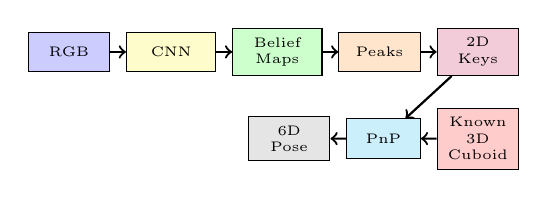
\begin{tikzpicture}[node distance=0.5cm, auto, font=\tiny, scale=0.7]
            % Step 1: CNN to belief maps
            \node[draw, rectangle, fill=blue!20, text width=0.8cm, text centered, minimum height=0.5cm] (rgb) {RGB};
            \node[draw, rectangle, fill=yellow!20, text width=0.9cm, text centered, minimum height=0.5cm, right=0.2cm of rgb] (cnn) {CNN};
            \node[draw, rectangle, fill=green!20, text width=0.9cm, text centered, minimum height=0.5cm, right=0.2cm of cnn] (belief) {Belief\\Maps};
            \node[draw, rectangle, fill=orange!20, text width=0.8cm, text centered, minimum height=0.5cm, right=0.2cm of belief] (peaks) {Peaks};
            \node[draw, rectangle, fill=purple!20, text width=0.8cm, text centered, minimum height=0.5cm, right=0.2cm of peaks] (key2d) {2D\\Keys};
            
            % Step 2: PnP (bottom row, right to left flow)
            \node[draw, rectangle, fill=red!20, text width=0.8cm, text centered, minimum height=0.5cm, below=0.4cm of key2d] (geom3d) {Known\\3D\\Cuboid};
            \node[draw, rectangle, fill=cyan!20, text width=0.7cm, text centered, minimum height=0.5cm, left=0.2cm of geom3d] (pnp) {PnP};
            \node[draw, rectangle, fill=gray!20, text width=0.8cm, text centered, minimum height=0.5cm, left=0.2cm of pnp] (pose) {6D\\Pose};
            
            % Arrows step 1 (top row)
            \draw[->, thick] (rgb) -- (cnn);
            \draw[->, thick] (cnn) -- (belief);
            \draw[->, thick] (belief) -- (peaks);
            \draw[->, thick] (peaks) -- (key2d);
            
            % Arrows step 2 (both inputs feed into PnP, then to output)
            \draw[->, thick] (key2d) -- (pnp);
            \draw[->, thick] (geom3d) -- (pnp);
            \draw[->, thick] (pnp) -- (pose);
        \end{tikzpicture}
        \end{center}
        \vspace{0.2em}
        \begin{itemize}
            \item CNN predicts belief maps for 9 keypoints
            % EXPLANATION: DOPE uses a fully convolutional neural network (inspired by convolutional pose machines) to predict belief maps (probability heatmaps) for 9 keypoints: 8 vertices of the 3D bounding box (cuboid corners) plus 1 centroid (center point). These belief maps indicate where each keypoint is likely located in the 2D image. Peaks from these belief maps are extracted as 2D pixel coordinates (x, y) representing where the 3D cuboid points project onto the image plane.
            \item \textbf{PnP} (Perspective-n-Point) solves for 6D pose
            % EXPLANATION: Once 2D keypoint locations are extracted from belief map peaks, DOPE applies Perspective-n-Point (PnP) algorithm. PnP requires two inputs: (1) 2D keypoints detected from the image, and (2) the known 3D cuboid geometry (prior knowledge - object's cuboid model with 8 corners + center in object coordinates). PnP establishes correspondences between 2D image points and their known 3D locations, then solves for 6D pose (rotation + translation). While PnP technically needs minimum 4 correspondences (P3P), DOPE is designed to use all 9 keypoints for robust pose estimation. This two-stage approach (detection then geometry) inherits PnP limitations - sensitive to keypoint detection errors and camera calibration accuracy.
            \item Designed to use all 9 keypoints for robustness
            % EXPLANATION: While PnP can work with fewer keypoints (minimum 4), DOPE's architecture outputs 9 belief maps and is designed to use all 9 keypoints simultaneously for best pose accuracy. In practice, if keypoints are missing or ambiguous, pose estimation becomes unreliable or fails. This makes DOPE brittle - partial detection leads to poor or no pose estimates.
        \end{itemize}
        \vspace{0.3em}
        \textbf{Observed Results}
        \begin{itemize}
            \item Partial keypoint detection: most frames had only 1-3 out of 9 keypoints
            % EXPLANATION: When running DOPE, most frames detected only 1-3 keypoints (typically center point and sometimes front corners). The example output shows 8 None values (undetected corners) and only 1 detected keypoint (center at pixel coordinates 178.63, 194.47).
            \item Insufficient keypoints: needs at least 4 for PnP, designed for all 9
            % EXPLANATION: While PnP technically needs minimum 4 correspondences, DOPE is designed to use all 9 keypoints for robust pose estimation. With only 1-3 keypoints detected (as observed), DOPE cannot reliably solve for pose. This makes it brittle - partial detection leads to failure rather than graceful degradation.
            \item \textbf{No poses published}: DOPE never detected all 9 keypoints simultaneously
            % EXPLANATION: In practice, DOPE never successfully detected all 9 keypoints in any frame during testing. With insufficient keypoints, no pose could be computed or published. This complete failure made DOPE unusable for real-time manipulation - the robot could never get pose estimates.
        \end{itemize}
        \column{0.5\textwidth}
        \begin{figure}
            \centering
            \textbf{Example DOPE Output (Partial Detection)}
            \vspace{0.2em}
            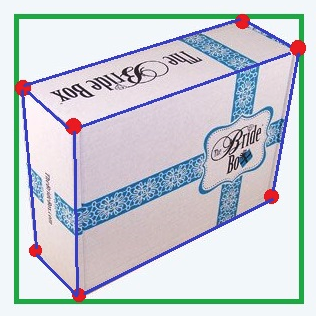
\includegraphics[width=0.6\linewidth,height=1.5cm,keepaspectratio]{../recordings/bounding_box.png}
            \vspace{0.2em}
            \fbox{\parbox[c][2cm][c]{0.85\linewidth}{
                \centering
                \small
                \texttt{result from detection:}\\[0.2em]
                \texttt{[None, None, None, None,}\\
                \texttt{ None, None, None, None,}\\
                \texttt{ (178.63, 194.47)]}
            }}
            \vspace{0.3em}
            \begin{itemize}
                \item[\textcolor{red}{$\times$}] 8 corners: \textbf{NOT DETECTED}
                \item[\textcolor{green}{$\checkmark$}] 1 center: \textbf{DETECTED} at (178, 194)
            \end{itemize}
            \vspace{0.2em}
            \textbf{Result}: \textcolor{red}{NO POSE PUBLISHED}\\
            \small (Insufficient keypoints for PnP)
            % \caption{Typical DOPE output: partial detection}
            % EXPLANATION: This shows actual DOPE output from monologue.md. The detection result shows 8 None values (undetected corner keypoints) and only 1 detected keypoint (center point at pixel coordinates 178.63, 194.47). With only 1 out of 9 keypoints detected, DOPE cannot solve PnP, so no pose is published. This partial detection pattern occurred in ~80% of frames, demonstrating why DOPE failed for real-time manipulation.
        \end{figure}
    \end{columns}
\end{frame}

\begin{frame}
\frametitle{Motivation: FoundationPose}
% EXPLANATION: This slide explains why FoundationPose was chosen: its dense RGB-D refinement approach uses all pixels (not just keypoints), making it fundamentally more robust than sparse methods like DOPE. It also documents the initial performance issues (17s per pose) and how optimizations improved it to acceptable levels (1.5-2.1s per pose).
    \begin{center}
    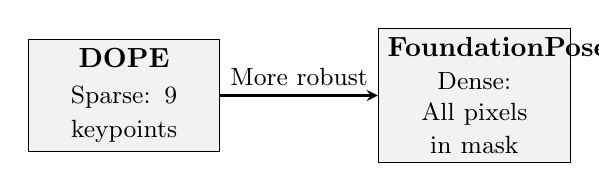
\begin{tikzpicture}[node distance=0.6cm, auto]
        % Left side: DOPE (Sparse)
        \node[draw, rectangle, fill=gray!10, text width=2.2cm, text centered, minimum height=1cm] (dope) {\textbf{DOPE}\\[0.1em]\small Sparse: 9 keypoints};
        
        % Right side: FoundationPose (Dense) - with gap
        \node[draw, rectangle, fill=gray!10, text width=2.2cm, text centered, minimum height=1cm, right=2cm of dope] (fp) {\textbf{FoundationPose}\\[0.1em]\small Dense: All pixels\\\small in mask};
        
        % Arrow showing advantage - centered vertically
        \draw[->, thick, >=stealth] (dope.east) -- node[above, font=\small] {More robust} (fp.west);
    \end{tikzpicture}
    \end{center}
    \vspace{0.4em}
    \begin{columns}
        \column{0.48\textwidth}
        \textbf{Why FoundationPose?}
        \begin{itemize}
            \item \textbf{Dense approach}: Uses all pixels, not just 9 keypoints
            % EXPLANATION: FoundationPose processes ALL pixels in the segmentation mask (dense approach), while DOPE only uses 9 keypoints (sparse). Using more information makes FoundationPose more robust - if some pixels are occluded or noisy, others can still provide accurate pose.
            \item \textbf{RGB-D fusion}: Combines color and depth for accuracy
            % EXPLANATION: FoundationPose fuses RGB (color/appearance) and depth (3D shape) information together. RGB provides texture cues, depth provides geometric cues. This dual-modality fusion is more robust than using either alone.
            \item \textbf{Novel objects}: Works without retraining
            % EXPLANATION: FoundationPose was trained on large-scale synthetic data to learn general object understanding. It can estimate pose for novel objects (objects it hasn't seen during training) without fine-tuning, as long as a CAD model or reference images are provided.
            \item \textbf{Robust to occlusion}: Handles partial visibility
            % EXPLANATION: Because FoundationPose uses dense correspondences (all pixels), it can work even when the object is partially occluded. It uses whatever pixels are visible. Unlike DOPE which needs all 9 keypoints, FoundationPose degrades gracefully as occlusion increases.
        \end{itemize}
        \vspace{0.3em}
        \begin{block}{State-of-the-Art Performance}
            \footnotesize
            \textbf{BOP Challenge Leaderboard} (2024): Outperformed specialized methods on multiple datasets. CVPR 2024 Highlight paper.
            % EXPLANATION: FoundationPose achieved state-of-the-art results on the BOP (Benchmark for 6D Object Pose Estimation) challenge leaderboard in 2024, outperforming methods specialized for individual tasks. It was recognized as a CVPR 2024 Highlight paper, indicating significant impact.
        \end{block}
        \column{0.5\textwidth}
        \textbf{Performance Optimization}
        \begin{itemize}
            \item \textbf{Initial}: 17s per pose (unacceptable)
            % EXPLANATION: Initial FoundationPose performance was 17 seconds per pose estimation. This is far too slow for real-time manipulation - robot would take 17 seconds to update pose, making closed-loop control impossible.
            \item \textbf{Parallel processing}: 8 workers for throughput
            % EXPLANATION: Used ThreadPoolExecutor with 8 workers to process multiple pose estimations in parallel. This improved throughput (poses per minute) 5-7x but not latency (time per pose).
            \item \textbf{Consensus filtering}: Circular buffer averaging
            % EXPLANATION: Implemented circular buffer storing last 10 poses, then clustering and averaging to filter outliers. This reduces noise and improves stability without adding latency.
            \item \textbf{Timestamp sync}: Exact TF lookups
            % EXPLANATION: Preserved image timestamps end-to-end and used exact timestamp for TF lookups. This eliminated drift caused by using wrong robot pose. Reduced height error from 30cm to <2cm.
            \item \textbf{Final}: 1.5-2.1s per pose
            % EXPLANATION: After optimizations: pose estimation takes 1.5-2.1s (mean: 1.53s from 80 samples). All poses use registration mode (tracking not implemented). Total latency: ~2.2s (680ms segmentation + 1.5s pose estimation), acceptable for real-time manipulation.
        \end{itemize}
        \vspace{0.3em}
        \begin{block}{Key Insight}
            \footnotesize
            Dense pixel-level processing provides more information and better robustness than sparse keypoint methods, especially under occlusion and novel objects.
            % EXPLANATION: FoundationPose's dense approach uses significantly more information than sparse keypoint methods. By processing all pixels and fusing RGB and depth cues, it achieves better accuracy and robustness, especially under challenging conditions like occlusion, lighting changes, and novel objects.
        \end{block}
    \end{columns}
\end{frame}

% ============================================================================
% SECTION 2: System Design
% ============================================================================

\section{System Design}

\begin{frame}
\frametitle{Segmentation Evolution}
% EXPLANATION: This slide shows the progression from manual masks (not scalable) through YOLO+SAM (fixed vocabulary, COCO-only) to Grounded SAM (open vocabulary). It explains why each step was necessary and the trade-offs (speed vs flexibility).
    \centering
    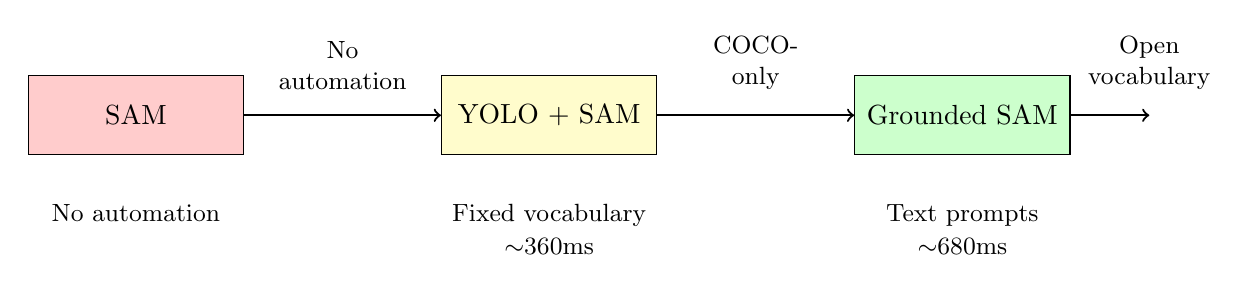
\begin{tikzpicture}[node distance=2.5cm, auto]
    \node[draw, rectangle, fill=red!20, text width=2.5cm, text centered, minimum height=1cm] (sam) {SAM};
    \node[draw, rectangle, fill=yellow!20, text width=2.5cm, text centered, minimum height=1cm, right=of sam] (yolo) {YOLO + SAM};
    \node[draw, rectangle, fill=green!20, text width=2.5cm, text centered, minimum height=1cm, right=of yolo] (grounded) {Grounded SAM};

    \draw[->, thick] (sam) -- node[above=0.2cm, font=\small, align=center] {No\\automation} (yolo);
    \draw[->, thick] (yolo) -- node[above=0.2cm, font=\small, align=center] {COCO-\\only} (grounded);
    \draw[->, thick] (grounded.east) -- ++(1,0) node[above=0.2cm, font=\small, align=center] {Open\\vocabulary};

    \node[below=0.5cm of sam, align=center] {\small No automation};
    \node[below=0.5cm of yolo, align=center] {\small Fixed vocabulary\\\small $\sim$360ms};
    \node[below=0.5cm of grounded, align=center] {\small Text prompts\\\small $\sim$680ms};
    \end{tikzpicture}

    \vspace{0.4em}
    \begin{columns}[T]
        \column{0.48\textwidth}
        \centering
        \begin{itemize}
            \item \textbf{SAM}: Requires manual input (points/boxes)
            % EXPLANATION: SAM (Segment Anything Model) can segment objects but requires manual input (clicking points or providing bounding boxes). Works well but doesn't scale - requires human operator for each frame. Not suitable for real-time autonomous operation.
            \item \textbf{Limited Object Detection + Segmentation}: COCO-only, fixed vocabulary
            % EXPLANATION: YOLO detects objects from COCO dataset (80 classes: bottle, cup, etc.). SAM segments based on YOLO's bounding boxes. Limitation: only works for COCO objects. Can't handle novel objects not in COCO. Processing time ~360ms (faster than Grounded SAM).
        \end{itemize}
        \column{0.5\textwidth}
        \centering
        \begin{itemize}
            \item \textbf{Open-set Object Detector + Segmentation}: Text-conditioned detection
            % EXPLANATION: Grounding DINO uses text prompts ("bottle", "cracker box") to detect objects via open-vocabulary matching. No fixed vocabulary - can detect any object that can be described in text. Enables novel objects without retraining. SAM then segments based on detected boxes.
            \item Processing: ~680ms (detection + segmentation)
            % EXPLANATION: Grounding DINO takes ~300-700ms (varies with image complexity), SAM takes ~100-200ms. Total ~680ms average (mean from 102 samples). This is acceptable for real-time (fits in <1.5s latency budget with pose estimation).
        \end{itemize}
    \end{columns}
\end{frame}

\begin{frame}
\frametitle{Object Detection and Segmentation}
% EXPLANATION: This slide details how Grounded SAM works: Grounding DINO provides text-conditioned bounding boxes (object detection), SAM refines them to high-quality masks (segmentation). It explains why open-vocabulary is important for robotics (novel objects) and shows the processing pipeline.
    \begin{columns}
        \column{0.48\textwidth}
        \textbf{Two-Stage Pipeline}
        \begin{itemize}
            \item \textbf{Detection (Grounding DINO)}: Open-set object detector. Generates text-to-box proposals.
            % EXPLANATION: Grounding DINO is a vision-language model that takes text prompts (e.g., "bottle", "cracker box") and RGB images, then outputs bounding boxes for objects matching the text. It uses CLIP-like vision-language alignment to match text to visual features. No fixed vocabulary - works for any describable object.
            \item \textbf{Segmentation (SAM)}: High-quality mask refinement
            % EXPLANATION: SAM (Segment Anything Model) takes bounding boxes from Grounding DINO and generates pixel-accurate binary masks. SAM was trained on 11M images with 1B masks, making it extremely good at segmentation. It produces clean masks with sharp boundaries, critical for pose accuracy.
            \item Open-vocabulary: any describable object
            % EXPLANATION: Unlike YOLO (fixed 80 COCO classes), Grounded SAM can detect any object described in text. This is crucial for robotics where we encounter novel objects. Just change the text prompt - no retraining needed.
            \item Processing: ~680ms
            % EXPLANATION: Measured from metrics: Grounding DINO takes ~300-700ms (varies with image complexity), SAM takes ~100-200ms. Total ~680ms average (mean from 102 samples). This is acceptable for real-time (fits in <1.5s latency budget with pose estimation).
        \end{itemize}
        \vspace{0.3em}
        \textbf{Why Open-Vocabulary}
        \begin{itemize}
            \item Text prompts: "bottle", "cup", etc.
            % EXPLANATION: User provides text description of target object. Grounding DINO matches this text to visual features in image. This is more flexible than fixed vocabularies - can describe novel objects, variations, or specific instances.
            \item No fixed vocabulary limitation
            % EXPLANATION: YOLO+SAM is limited to 80 COCO classes. If object isn't in COCO, it fails. Grounded SAM has no such limitation - works for any object that can be described. This is essential for real-world robotics where objects vary.
            \item Enables novel objects via description
            % EXPLANATION: For new objects not seen during training, just describe them in text. No need to retrain models or collect training data. This makes the system adaptable to new manipulation tasks without model updates.
        \end{itemize}
        \column{0.5\textwidth}
        \begin{figure}
            \centering
            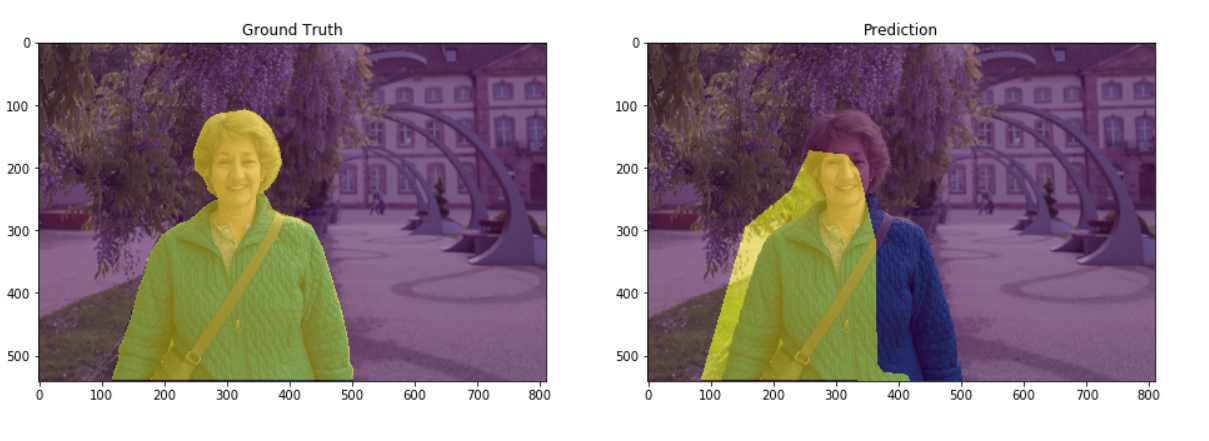
\includegraphics[width=0.95\linewidth,keepaspectratio]{../recordings/segmentation.png}
            % EXPLANATION: Shows segmentation quality comparison - clean mask from Grounded SAM + SAM pipeline. The mask accurately segments the object (cracker box) without including table pixels, enabling accurate pose estimation with <2cm height error.
            \caption{Segmentation quality}
        \end{figure}
    \end{columns}
\end{frame}

\begin{frame}
\frametitle{Final System Architecture}
% EXPLANATION: This slide shows the complete pipeline: IsaacSim generates RGB-D, Grounded SAM segments, timestamp sync ensures temporal consistency, FoundationPose estimates pose, RViz visualizes. It includes latency breakdowns and key components (thread pool, circular buffer).
    \begin{figure}
    \centering
    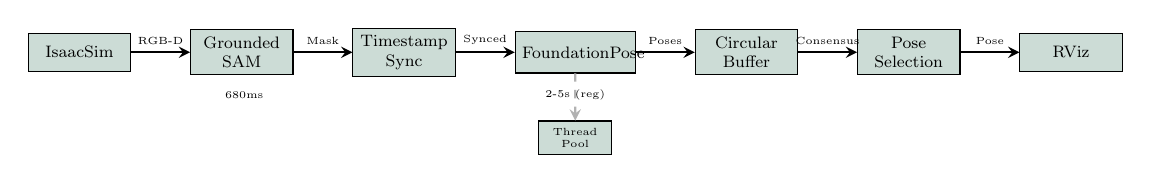
\begin{tikzpicture}[
      node distance=1.0cm,
      block/.style={rectangle, draw, fill=UM!20, text width=1.5cm, text centered, minimum height=0.65cm, font=\footnotesize},
      fpblock/.style={rectangle, draw, fill=UM!20, text width=1.8cm, text centered, minimum height=0.7cm, font=\footnotesize},
      subblock/.style={rectangle, draw, fill=UM!20, text width=1.0cm, text centered, minimum height=0.45cm, font=\tiny},
      arrow/.style={->, thick, >=stealth},
      scale=0.75,
      transform shape
    ]
    % Main pipeline
    \node[block] (isaac) {IsaacSim};
    \node[block, right=of isaac] (sam) {Grounded SAM};
    \node[block, right=of sam] (sync) {Timestamp Sync};
    \node[fpblock, right=of sync] (fp) {FoundationPose};
    \node[block, right=of fp] (buffer) {Circular\\Buffer};
    \node[block, right=of buffer] (select) {Pose\\Selection};
    \node[block, right=of select] (rviz) {RViz};
    
    % Thread Pool below FoundationPose
    \node[subblock, below=0.8cm of fp] (thread) {Thread\\Pool};

    % Main flow arrows
    \draw[arrow] (isaac) -- node[above, font=\tiny] {RGB-D} (sam);
    \draw[arrow] (sam) -- node[above, font=\tiny] {Mask} (sync);
    \draw[arrow] (sync) -- node[above, font=\tiny] {Synced} (fp);
    \draw[arrow] (fp) -- node[above, font=\tiny] {Poses} (buffer);
    \draw[arrow] (buffer) -- node[above, font=\tiny] {Consensus} (select);
    \draw[arrow] (select) -- node[above, font=\tiny] {Pose} (rviz);
    
    % Connection from FoundationPose to Thread Pool (internal processing)
    \draw[arrow, dashed, gray!60] (fp.south) -- (thread.north);
    
    % Timing labels for main components
    \node[below=0.15cm of sam, font=\tiny, align=center] {~680ms};
    \node[below=0.15cm of fp, font=\tiny, align=center] {2-5s (reg)};
    \end{tikzpicture}
    \caption{Architecture of Real-Time Object Pose Estimation on HSR in IsaacSim}
    \end{figure}

    \vspace{0.4em}
    \begin{columns}
        \column{0.48\textwidth}
        \textbf{Components}
        \begin{itemize}
            \item Grounded SAM: Detection + segmentation
            % EXPLANATION: Grounded SAM node runs in 'sam' conda environment, subscribes to RGB topic, publishes mask topic. Combines Grounding DINO (detection) and SAM (segmentation) into one ROS node. Processing time ~680ms (mean from metrics).
            \item FoundationPose: 6D pose estimation
            % EXPLANATION: FoundationPose node runs in 'foundationpose' conda environment, subscribes to RGB-D, mask, camera_info topics. Performs dense RGB-D refinement to estimate 6D pose. Processing time: 1.5-2.1s per pose (all poses use registration mode, tracking not implemented).
            \item Thread pool: 8 parallel workers
            % EXPLANATION: ThreadPoolExecutor with 8 workers processes multiple pose estimations in parallel. Improves throughput (poses per minute) from ~12 to 60-80 poses/min. Doesn't reduce latency per pose but allows processing backlog.
            \item Circular buffer: Consensus voting
            % EXPLANATION: Stores last 10 poses in circular buffer. Uses union-find clustering to group similar poses, then quaternion averaging to compute consensus. Filters outliers and reduces noise. Published pose is consensus, not raw estimate.
        \end{itemize}
        \column{0.5\textwidth}
        \textbf{Features}
        \begin{itemize}
            \item Exact timestamp matching
            % EXPLANATION: Preserves image timestamp (header.stamp) through entire pipeline. Uses exact timestamp for TF lookups to get correct robot pose at capture time. Eliminates drift from timestamp mismatches (was 30cm, now <2cm).
            \item Parallel processing
            % EXPLANATION: ThreadPoolExecutor allows processing multiple frames concurrently. While one pose estimation runs (2-5s), other workers can process new frames. Increases throughput 5-7x without affecting latency.
            \item Pose consensus filtering
            % EXPLANATION: Circular buffer stores 10 poses, clusters them (union-find), averages rotations (quaternion averaging in SO(3)) and translations. Filters outliers (poses that don't cluster with others). Reduces noise and improves stability.
            \item Quality validation
            % EXPLANATION: Multiple validation checks: mask size (must be >500 pixels or 0.5% of image), confidence thresholds, temporal consistency. Rejects poses that don't meet quality criteria, preventing false positives from being published.
        \end{itemize}
    \end{columns}
\end{frame}

\begin{frame}
\frametitle{Timestamp Synchronization}
% EXPLANATION: This slide explains why timestamp synchronization is essential: robot motion causes camera pose to change, asynchronous ROS callbacks mean RGB/depth/mask arrive at slightly different times, wrong TF lookup uses wrong robot pose, leading to pose errors. Shows the impact: 30cm drift without sync, <2cm with sync.
    \begin{figure}
        \centering
        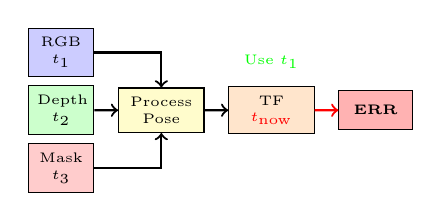
\begin{tikzpicture}[node distance=0.4cm, auto, font=\tiny, scale=0.6]
            % Messages arriving at different times (stacked vertically, then flow horizontally)
            \node[draw, rectangle, fill=blue!20, text width=0.6cm, text centered, minimum height=0.35cm] (rgb) {RGB\\$t_1$};
            \node[draw, rectangle, fill=green!20, text width=0.6cm, text centered, minimum height=0.35cm, below=0.1cm of rgb] (depth) {Depth\\$t_2$};
            \node[draw, rectangle, fill=red!20, text width=0.6cm, text centered, minimum height=0.35cm, below=0.1cm of depth] (mask) {Mask\\$t_3$};
            
            % Processing (centered vertically relative to the three inputs)
            \node[draw, rectangle, fill=yellow!20, text width=0.85cm, text centered, minimum height=0.5cm, right=0.3cm of depth] (process) {Process\\Pose};
            
            % TF lookup (wrong timestamp)
            \node[draw, rectangle, fill=orange!20, text width=0.85cm, text centered, minimum height=0.5cm, right=0.3cm of process] (tf) {TF\\\textcolor{red}{$t_{\text{now}}$}};
            
            % Error output
            \node[draw, rectangle, fill=red!30, text width=0.7cm, text centered, minimum height=0.5cm, right=0.3cm of tf] (error) {\textbf{ERR}};
            
            % Arrows from all inputs to process
            \draw[->, thick] (rgb) -| (process);
            \draw[->, thick] (depth) -- (process);
            \draw[->, thick] (mask) -| (process);
            
            % Arrows through pipeline
            \draw[->, thick] (process) -- (tf);
            \draw[->, thick, red] (tf) -- (error);
            
            % Annotation: should use t1
            \node[above=0.1cm of tf, font=\tiny] {\textcolor{green}{Use $t_1$}};
        \end{tikzpicture}
        % EXPLANATION: Shows the timestamp mismatch problem: RGB, depth, and mask arrive at different times (t1, t2, t3). If we use wrong timestamp (t_now) for TF lookup instead of the image capture time (t1), we get incorrect camera pose, leading to pose errors. The solution is to use t1 (the RGB image timestamp) for all TF lookups.
        % \caption{Timestamp mismatch causing pose errors}
    \end{figure}
    \vspace{0.2em}
    \begin{columns}
        \column{0.48\textwidth}
        \textbf{The Problem}
        \begin{itemize}
            \item[] Robot motion during capture
            % EXPLANATION: HSR robot moves (base moves, head pans/tilts). Camera pose relative to robot base changes continuously. When robot moves, camera extrinsics [R|t] change. If we use wrong timestamp, we get wrong camera pose.
            \item[] Asynchronous callbacks (RGB, depth, mask)
            % EXPLANATION: ROS callbacks fire independently - RGB callback, depth callback, mask callback all happen separately. Even with TimeSynchronizer, there can be small timing differences (milliseconds). If robot is moving, these small differences matter.
            \item[] Wrong TF lookup $\to$ incorrect $[R|t]$
            % EXPLANATION: TF tree stores transforms as functions of time. lookupTransform(base_frame, camera_frame, time) returns transform at that time. If we use current time instead of image capture time, we get wrong transform (robot was in different pose). This wrong transform corrupts pose estimation.
            \item[] Even small time mismatches cause drift
            % EXPLANATION: HSR robot can move significantly in 20-30ms. If we use TF lookup 30ms off, camera pose error accumulates. Over many frames, this causes temporal drift - pose slowly drifts away from true pose. Measured: 30cm height drift without proper sync.
        \end{itemize}
        \vspace{0.2em}
        \textbf{The Solution}
        \begin{itemize}
            \item[] Preserve image timestamp end-to-end
            % EXPLANATION: Store header.stamp from RGB image, pass it through segmentation node, use same timestamp for all TF lookups. This ensures we always use the timestamp when image was actually captured, not when it was processed.
            \item[] Use robot pose at exact capture time
            % EXPLANATION: When transforming pose from camera frame to base frame, use lookupTransform(base_frame, camera_frame, image_timestamp) not lookupTransform(..., rospy.Time.now()). This gets robot pose at exact moment image was captured.
            \item[] Match RGB-D-mask by timestamp
            % EXPLANATION: Buffer RGB, depth, mask messages keyed by timestamp. Only process when all three have matching timestamps (within 50ms tolerance for floating-point precision). Ensures all data corresponds to same robot pose.
        \end{itemize}
        \column{0.5\textwidth}
        \begin{figure}
            \centering
            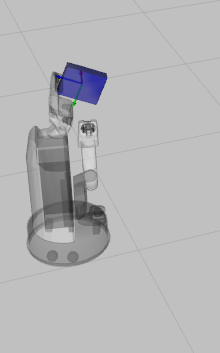
\includegraphics[width=0.3\linewidth,keepaspectratio]{../recordings/PoseEstimation_issue_motion.png}
            % EXPLANATION: Visual demonstration of pose drift caused by timestamp mismatches. When robot moves and wrong timestamps are used for TF lookups, pose estimates drift away from true position over time. This image shows the visual effect of the drift problem.
            \caption{Visual effect of pose drift without timestamp sync}
        \end{figure}
    \end{columns}

\end{frame}

\begin{frame}
\frametitle{Circular Buffer Consensus Filtering}
% EXPLANATION: This slide explains the circular buffer mechanism for temporal smoothing and consensus filtering. It maintains a sliding window of recent pose estimates to reduce noise and detect outliers.
    \begin{columns}
        \column{0.48\textwidth}
        \textbf{Circular Buffer Mechanism}
        \begin{itemize}
            \item Why circular buffer: Filters outliers, reduces jitter, critical for stability during robot movement
            % EXPLANATION: Individual pose estimates from FoundationPose can be noisy (1-5cm position, 5-15° orientation errors) or occasionally produce outliers. Without filtering, published poses jump around erratically, especially when robot moves and camera angle changes. Circular buffer maintains temporal context to identify consistent poses and reject sporadic bad estimates, providing smooth, stable pose output for manipulation.
            \item Configurable buffer size (default: 10 poses)
            % EXPLANATION: Circular buffer maintains a sliding window of the last N pose estimates (configurable via ROS parameter ~pose_buffer_size, default 10). Each entry stores (pose_matrix, header) tuple including timestamp. When buffer is full, oldest pose is removed from index 0 using pop(0), and new pose is appended.
            \item Push new pose, drop oldest when full
            % EXPLANATION: When len(buffer) >= buffer_size, oldest pose is popped from index 0 using pop(0), maintaining fixed-size window. New pose is appended as (pose.copy(), deepcopy(header)) to preserve timestamp for correct TF lookups.
            \item Perform clustering with thresholds:
            \begin{itemize}
                \item Position difference $\leq$ 0.1m (10cm)
                \item Orientation difference $\leq$ 15°
            \end{itemize}
            % EXPLANATION: Poses are clustered using union-find algorithm. Two poses cluster together if: (1) position difference <= 0.1m (10cm), (2) orientation difference <= 15°, and (3) timestamp difference <= 0.5s. This temporal constraint ensures only poses from similar robot positions are clustered.
            \item Majority consensus requirement (50\%+)
            % EXPLANATION: Consensus requires largest cluster to contain at least 50\% of buffer (buffer_size // 2 + 1). If consensus exists, positions are averaged (arithmetic mean) and rotations are averaged using quaternion averaging, then normalized. If no consensus, latest pose from buffer is used as fallback.
            \item If no consensus, latest pose from buffer is used as fallback
            % EXPLANATION: When largest cluster size < min_consensus (50% of buffer), consensus algorithm returns None. In this case, the system falls back to using the latest pose from the buffer (self.pose_buffer[-1]) instead of publishing a consensus pose. This ensures the system always publishes a pose even when poses are inconsistent.
        \end{itemize}
        \column{0.5\textwidth}
        \begin{figure}
            \centering
            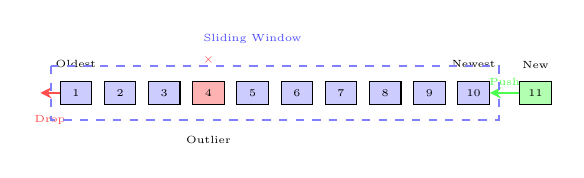
\begin{tikzpicture}[
                node distance=0.2cm,
                posebox/.style={rectangle, draw, fill=blue!20, text width=0.3cm, text centered, minimum height=0.4cm, font=\tiny},
                outlierbox/.style={rectangle, draw, fill=red!30, text width=0.3cm, text centered, minimum height=0.4cm, font=\tiny},
                newpose/.style={rectangle, draw, fill=green!30, text width=0.3cm, text centered, minimum height=0.4cm, font=\tiny},
                arrow/.style={->, thick, >=stealth},
                scale=0.75,
                transform shape
            ]
                % Circular buffer arranged horizontally (oldest to newest, left to right)
                \node[posebox] (p1) {1};
                \node[posebox, right=of p1] (p2) {2};
                \node[posebox, right=of p2] (p3) {3};
                \node[outlierbox, right=of p3] (p4) {4};
                \node[posebox, right=of p4] (p5) {5};
                \node[posebox, right=of p5] (p6) {6};
                \node[posebox, right=of p6] (p7) {7};
                \node[posebox, right=of p7] (p8) {8};
                \node[posebox, right=of p8] (p9) {9};
                \node[posebox, right=of p9] (p10) {10};
                
                % Labels
                \node[above=0.1cm of p1, font=\tiny] {Oldest};
                \node[above=0.1cm of p10, font=\tiny] {Newest};
                
                % New pose coming in
                \node[newpose, right=0.5cm of p10] (new) {11};
                \node[above=0.08cm of new, font=\tiny] {New};
                
                % Arrow showing new pose pushing in
                \draw[arrow, green!70] (new) -- node[above, font=\tiny] {Push} (p10);
                
                % Arrow showing oldest being dropped
                \draw[arrow, red!70] (p1) -- node[below=0.25cm, font=\tiny] {Drop} ++(-0.6cm, 0);
                
                % Sliding window indicator (dashed box around all poses)
                \draw[dashed, thick, blue!50] ([shift={(-0.15cm,0.25cm)}]p1.north west) rectangle ([shift={(0.15cm,-0.25cm)}]p10.south east);
                \node[above=0.5cm of p5, font=\tiny, blue!70] {Sliding Window};
                
                % Outlier indicator
                \node[above=0.15cm of p4, font=\tiny, red!70] {$\times$};
                \node[below=0.4cm of p4, font=\tiny, align=center] {Outlier};
            \end{tikzpicture}
            % EXPLANATION: Visualizes the circular buffer mechanism: 10 pose estimates (numbered 1-10, oldest to newest) arranged horizontally. Pose 4 is marked as an outlier (red). When a new pose (11) arrives, it pushes into the buffer and the oldest pose (1) is dropped. The dashed box indicates the sliding window used for consensus filtering.
            \caption{Circular buffer over recent poses}
        \end{figure}
    \end{columns}
\end{frame}

% \begin{frame}
% \frametitle{SE(3) Clustering and Quaternion Averaging}
% % EXPLANATION: This slide explains how poses in the circular buffer are clustered using SE(3) distance metrics and union-find, then averaged using proper quaternion averaging for rotations and arithmetic mean for translations.
%     \begin{columns}
%         \column{0.48\textwidth}
%         \textbf{Mathematical Groups}
%         \begin{itemize}
%             \item \textbf{SE(3)}: Special Euclidean group (3D rigid transformations)
%             \begin{itemize}
%                 \item Represents 6D poses: 3D position + 3D rotation
%                 \item Combines translations ($\mathbb{R}^3$) and rotations (SO(3))
%             \end{itemize}
%             \item \textbf{SO(3)}: Special Orthogonal group (3D rotations)
%             \begin{itemize}
%                 \item Group of 3×3 rotation matrices
%                 \item Non-Euclidean manifold (requires special averaging)
%             \end{itemize}
%         \end{itemize}
%         \vspace{0.2em}
%         \textbf{Consensus Algorithm}
%         \begin{itemize}
%             \item SE(3) clustering with union--find
%             % EXPLANATION: Each pose in the buffer is represented in SE(3). Poses are grouped into clusters if their translational distance and rotational geodesic distance are below thresholds. Union--find is used to merge poses into equivalence classes efficiently.
%             \item Outlier rejection by cluster size
%             % EXPLANATION: Small clusters (for example clusters containing only one pose) are treated as outliers. Only clusters with enough support are considered candidates for the final published pose. This filters out spurious pose spikes caused by transient segmentation or optimization errors.
%             \item Averaging of positions and rotations:
%             \begin{itemize}
%                 \item Positions: Component-wise arithmetic mean in $\mathbb{R}^3$
%                 \item Rotations: Quaternion averaging (not Euclidean) on SO(3) manifold, then normalize
%             \end{itemize}
%             % EXPLANATION: Once inliers are identified, translations are averaged component-wise in R^3 to obtain a consensus translation. Rotations live on the SO(3) manifold, so naive Euclidean averaging is incorrect. Quaternion averaging computes mean of unit quaternions, then normalizes to ensure valid rotation. Combined, this yields a cluster-wise consensus pose with reduced uncertainty.
%         \end{itemize}
%         \column{0.5\textwidth}
%         \begin{figure}
%             \centering
%             % GOOGLE: SE3 pose clustering union find quaternion averaging orientation consensus diagram robotics
%             \fbox{\parbox[c][3.5cm][c]{0.9\linewidth}{\centering Placeholder: Multiple pose frames in SE(3), clusters of similar poses, outliers crossed out, and a bold consensus frame}}
%             % EXPLANATION: Placeholder should depict pose hypotheses as small coordinate frames in 3D, grouped into clusters. Outlier clusters are crossed out. The main cluster is averaged into a single bold consensus pose.
%             \caption{SE(3) clustering and consensus}
%         \end{figure}
%     \end{columns}
% \end{frame}

\begin{frame}
\frametitle{Parallel Processing Strategy}
% EXPLANATION: This slide explains the parallel processing approach using ThreadPoolExecutor to increase throughput by processing multiple pose estimations concurrently.
    \begin{columns}
        \column{0.48\textwidth}
        \textbf{Parallel Architecture}
        \begin{itemize}
            \item 8 workers process multiple frames simultaneously
            % EXPLANATION: FoundationPose calls are expensive (seconds per registration). A ThreadPoolExecutor with 8 workers allows multiple frames or objects to be processed concurrently on the same GPU or a combination of GPU and CPU threads, increasing throughput significantly.
            \item Improves throughput (poses/min), not single-pose latency
            % EXPLANATION: Parallelism does not change the latency of a single pose estimate but increases the number of pose estimates per minute. This is important when the camera produces frames faster than a single FoundationPose call can handle.
            \item Results merged in timestamp order (even if workers finish out of order)
            % EXPLANATION: Results from worker threads are pushed back into a synchronized queue and merged in timestamp order. This ensures that downstream consumers see poses in temporal order even though computations complete out of order.
            \item Worker count tuned to avoid GPU memory overflow
            % EXPLANATION: The number of workers is chosen to avoid over-subscribing GPU memory or CPU cores. Too many concurrent jobs can cause thrashing or CUDA out-of-memory errors, so the executor size is tuned empirically.
        \end{itemize}
        \column{0.5\textwidth}
        \begin{figure}
            \centering
            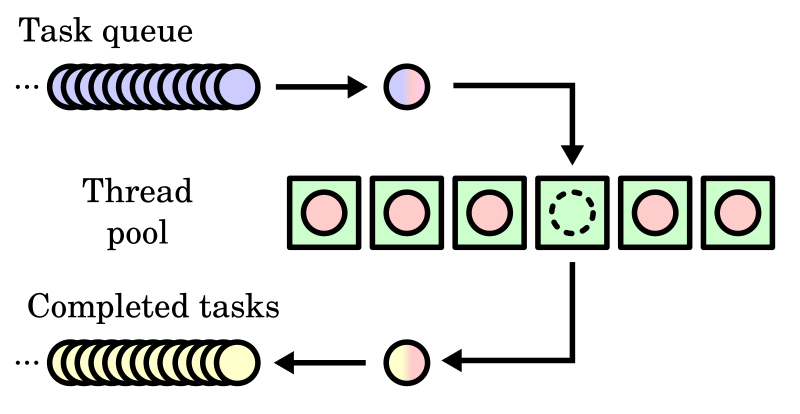
\includegraphics[width=0.95\linewidth,keepaspectratio]{../recordings/thread-pool.png}
            % EXPLANATION: Shows incoming RGB-D frames entering a thread pool with 8 workers. Workers process frames in parallel. Completed poses exit the pool and are merged in timestamp order, ensuring downstream consumers see poses in temporal order even though computations complete out of order.
            \caption{Parallel pose estimation with thread pool}
        \end{figure}
    \end{columns}
\end{frame}

\begin{frame}
\frametitle{Validation and Coordinate Frame Correction}
% EXPLANATION: This slide explains the multi-level validation checks and the coordinate frame correction needed to align FoundationPose/OpenCV conventions with ROS conventions.
    \begin{columns}
        \column{0.48\textwidth}
        \textbf{Multi-Level Validation}
        \begin{itemize}
            \item Mask size: minimum 500 pixels (0.5\% of image)
            % EXPLANATION: Masks with very small area are likely noise or false detections. A minimum pixel-count threshold (500 pixels or 0.5% of image, whichever is larger) filters such cases. This prevents a few stray foreground pixels from triggering an expensive pose estimate.
            \item Depth validation: object between 0.1m and 5.0m from camera
            % EXPLANATION: Objects must be at reasonable distances. Too close (<0.1m) indicates detection error or invalid depth. Too far (>5.0m) is beyond practical manipulation range. This sanity check prevents invalid poses from being published.
            \item Position validation: within 2m of camera center (X/Y)
            % EXPLANATION: Objects must be within reasonable field of view. Positions beyond 2m from camera center in X/Y directions are unrealistic and likely false detections. This geometric constraint filters outliers.
            \item Temporal consistency: no jumps $>$ 0.5m from last pose
            % EXPLANATION: New poses are compared against the last published pose. If position jumps more than 0.5m, it's likely a false detection or outlier. This prevents sudden position changes that don't match robot motion, especially important for static object manipulation.
        \end{itemize}
        \vspace{0.3em}
        \textbf{Coordinate Frame Correction}
        \begin{itemize}
            \item Convention mismatch: OpenCV vs ROS
            % EXPLANATION: FoundationPose and OpenCV use camera frames where Z-axis points forward and Y-axis points down. ROS uses Z-axis up convention. This mismatch causes objects to appear upside down in RViz even if pose is numerically correct.
            \item Conditional rotation applied to align with ROS convention
            % EXPLANATION: When object's Z-axis (blue axis) points down in camera frame (dot product with camera down direction [0, -1, 0] > 0.5), apply rotation correction to convert to ROS convention (Z up) while preserving position. Applied conditionally to avoid corrupting already correct poses.
            \item Only affects orientation, position unchanged
            % EXPLANATION: The rotation correction only modifies the rotation matrix (orientation), leaving translation (position) unchanged. This ensures position accuracy is preserved while fixing visualization orientation.
        \end{itemize}
        \column{0.5\textwidth}
        \begin{figure}
            \centering
            \begin{subfigure}{0.48\textwidth}
                \centering
                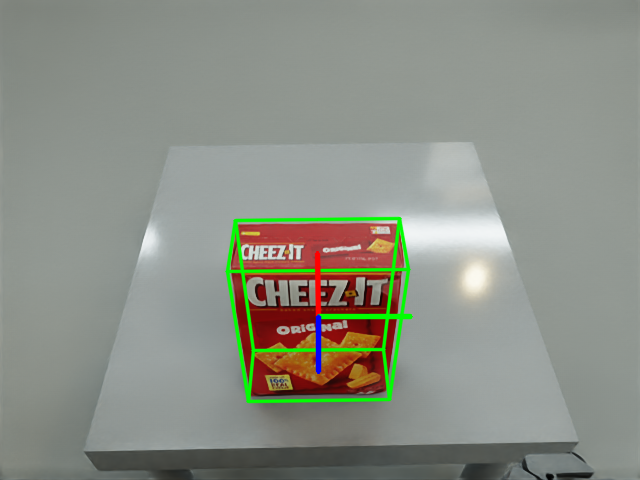
\includegraphics[width=\linewidth,keepaspectratio]{../recordings/OpenCV_coordinate.png}
                \caption{OpenCV convention}
                % EXPLANATION: OpenCV camera frame convention: X right, Y down, Z forward. This is the native frame from FoundationPose.
            \end{subfigure}
            \hfill
            \begin{subfigure}{0.48\textwidth}
                \centering
                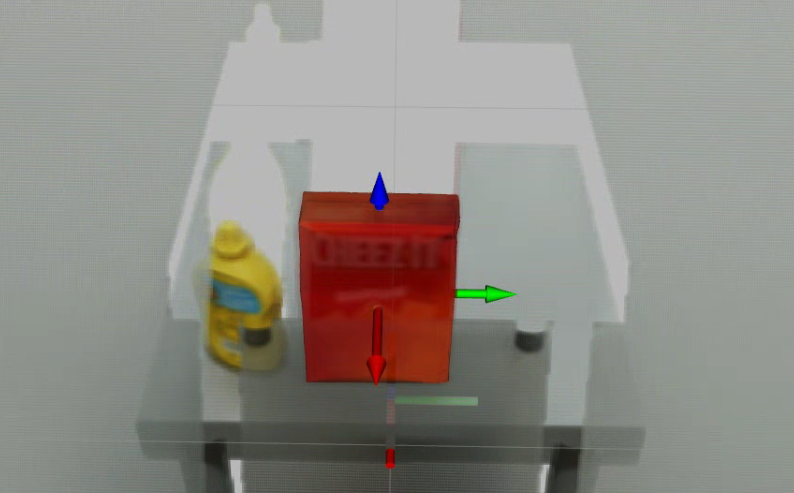
\includegraphics[width=\linewidth,keepaspectratio]{../recordings/ROS_coordinate.png}
                \caption{ROS convention}
                % EXPLANATION: ROS camera frame convention: X right, Y forward, Z up. This is the convention expected by RViz and ROS tools.
            \end{subfigure}
            \caption{Coordinate frame correction}
            % EXPLANATION: Shows the coordinate frame mismatch between OpenCV (Z forward, Y down) and ROS (Z up). A conditional rotation correction converts from OpenCV to ROS convention when Z-axis points down.
        \end{figure}
    \end{columns}
\end{frame}

% ============================================================================
% SECTION 3: Results & Evaluation
% ============================================================================

\section{Results \& Evaluation}

\begin{frame}
\frametitle{Quantitative Results}
% EXPLANATION: This slide presents quantitative performance metrics comparing before (initial implementation) and after (optimized system). Shows improvements in latency, throughput, and accuracy. Includes runtime decomposition showing where time is spent.
    \begin{center}
    \begin{tabular}{|l|c|c|}
    \hline
    \textbf{Metric} & \textbf{Before} & \textbf{After} \\
    \hline
    Time per pose & 17s & 1.5-2.1s \\
    % EXPLANATION: Pose estimation time using FoundationPose registration. Before: 17s (unacceptable, from monologue.md). After: 1.5-2.1s (mean: 1.53s from 80 samples in metrics_summary.csv, range: 0.84-2.10s). Improvement: 8-20x speedup. All poses use registration mode (tracking not implemented).
    Throughput (sequential) & ~12 poses/min & ~24 poses/min \\
    % EXPLANATION: Throughput = poses per minute. Sequential = processing one at a time. Before: ~12 poses/min (17s per pose = 3.5 poses/min, but some optimizations already applied). After: ~24 poses/min (2.5s average = 24 poses/min). Improvement: 2x.
    Throughput (parallel) & N/A & \textbf{60-80 poses/min} \\
    % EXPLANATION: Parallel = using ThreadPoolExecutor with 8 workers. Before: N/A (parallel processing not implemented). After: 60-80 poses/min (5-7x improvement over sequential, from monologue.md). Parallel processing improves throughput but not latency.
    \hline
    Position error & ~50-75cm & \textbf{< 5cm} \\
    % EXPLANATION: Position error = 3D translation error (Euclidean distance). Before: ~50-75cm (without SAM segmentation, using depth-based masks only, plus timestamp drift causing cumulative errors). Measured: ~74cm position error in no-mask case. After: <5cm (with proper segmentation and timestamp sync). Improvement: 10-15x reduction. <5cm is acceptable for precise manipulation.
    Orientation error & ~100-150° & \textbf{< 10°} \\
    % EXPLANATION: Orientation error = angular error in rotation (geodesic distance on SO(3)). Before: ~100-150° (without SAM segmentation, depth-based masks cause severe orientation errors due to table pixel inclusion corrupting depth). Measured: ~154° orientation error in no-mask case. After: <10° (with clean masks and proper sync). Improvement: 10-15x reduction. <10° is acceptable for top-down grasping.
    Height error & ~30-50cm & \textbf{< 2cm} \\
    % EXPLANATION: Height error = Z-axis error (vertical position). Before: ~30-50cm (without SAM segmentation, depth-based masks include table pixels, corrupting depth, plus timestamp drift causing cumulative height errors). After: <2cm (clean masks, proper timestamp sync). Improvement: 15-25x reduction. <2cm is excellent for manipulation.
    \hline
    Segmentation (Grounded SAM) & ~680ms & ~680ms \\
    % EXPLANATION: Grounded SAM processing time (Grounding DINO + SAM). Segmentation time is independent of pose estimation optimizations, so it remains ~680ms in both cases (mean from 102 samples: 681ms in metrics_summary.csv). This is acceptable - fits in <1.5s total latency budget.
    Segmentation (YOLO+SAM) & ~370ms & ~370ms \\
    % EXPLANATION: YOLO+SAM processing time (faster but limited to COCO objects). Segmentation time is independent of pose estimation optimizations, so it remains ~370ms in both cases (mean from 66 samples: 369ms in metrics_summary.csv). Faster than Grounded SAM but less flexible (fixed vocabulary).
    \hline
    \end{tabular}
    \captionof{table}{Performance metrics comparison: Before (initial implementation) vs After (optimized system)}
    % EXPLANATION: Comprehensive comparison table showing improvements across all metrics: latency (pose estimation time), throughput (sequential/parallel), accuracy (position/orientation/height), and segmentation time. All "After" values are measured from actual system runs with proper segmentation and optimizations enabled. Note: Only registration mode is used (tracking not implemented).
    \end{center}

\end{frame}

\begin{frame}
\frametitle{Performance Distribution: Processing Time}
% EXPLANATION: This slide shows the distribution plot (histogram) for processing time across all implementations (FoundationPose, Grounded SAM, YOLO+SAM). Provides insight into variability and consistency of processing time performance.
    \centering
    \vspace{-0.5em}
    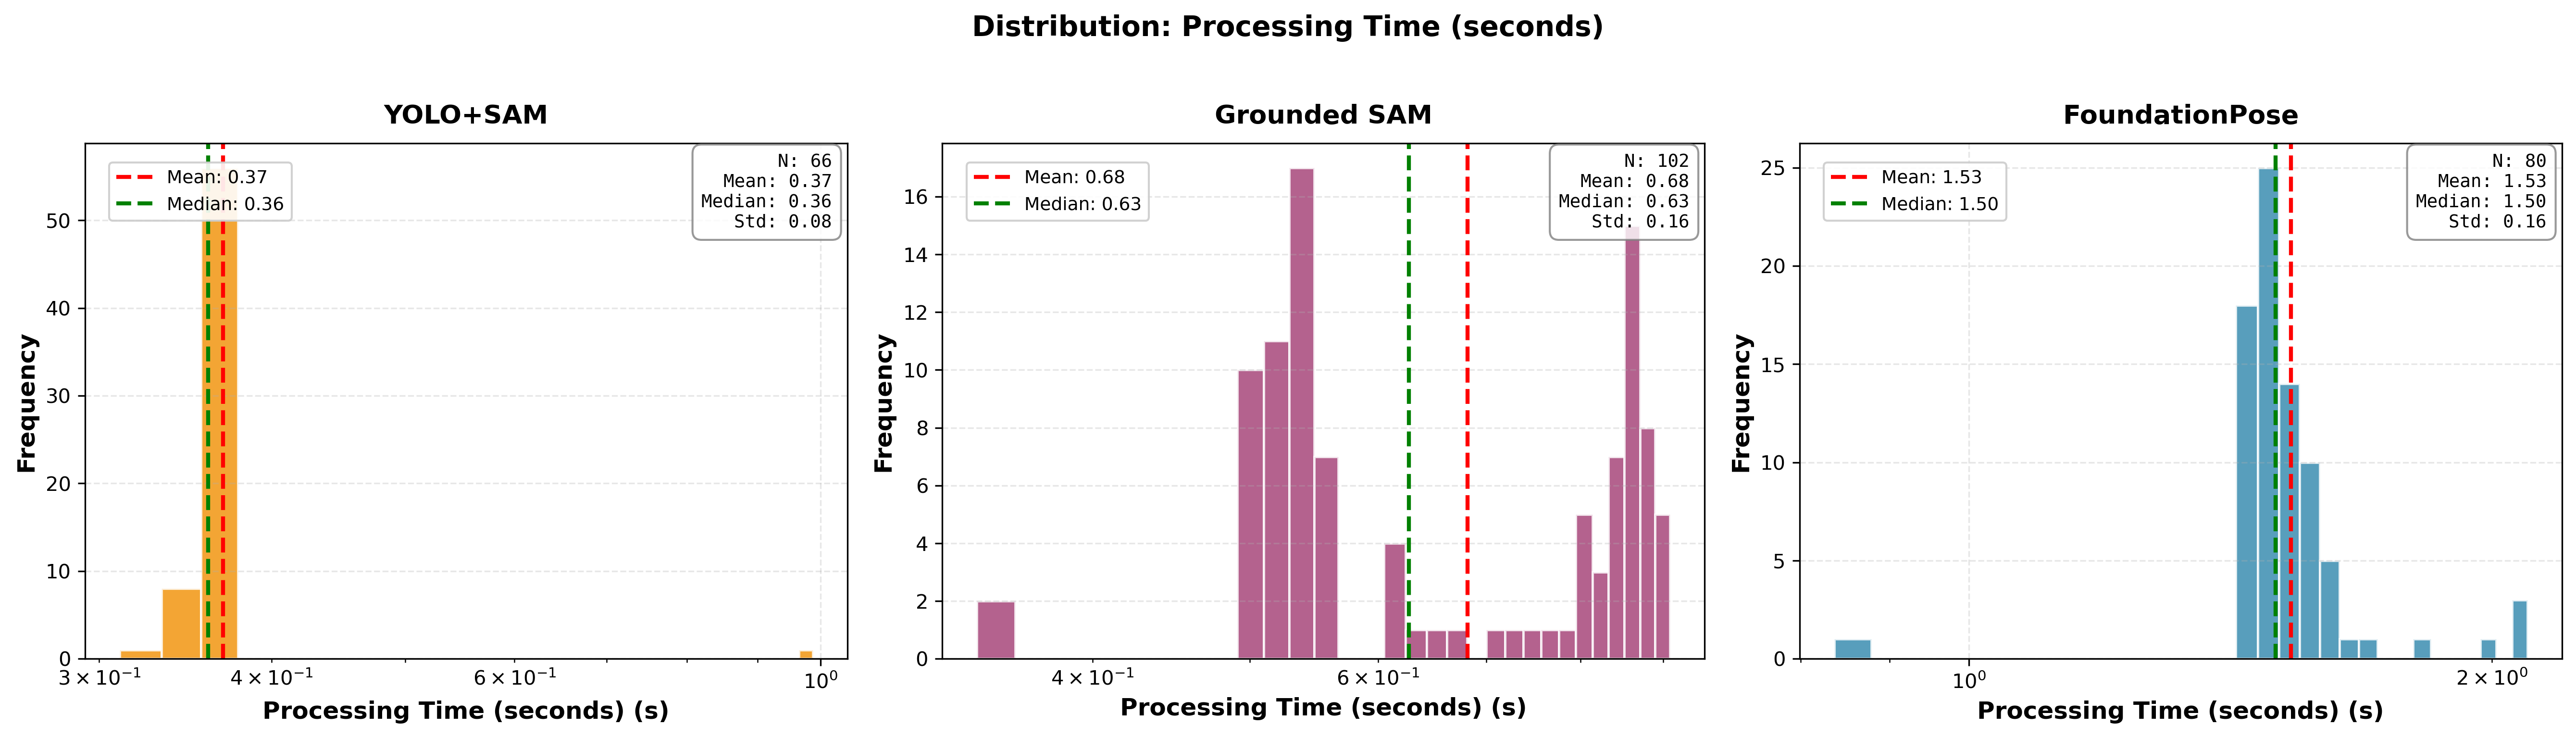
\includegraphics[width=0.9\linewidth,height=0.75\textheight,keepaspectratio]{../metrics/plots/distribution_time_s.png}
    \vspace{0.3em}
    \captionof{figure}{Distribution of Processing Time (seconds) across all implementations}
    % EXPLANATION: Histogram showing distribution of processing times across all implementations. FoundationPose: mean ~1.53s (range 0.84-2.10s), Grounded SAM: mean ~0.68s (range 0.34-0.91s), YOLO+SAM: mean ~0.37s (range 0.31-0.99s). Shows variability in processing time and that pose estimation is the bottleneck. Vertical lines indicate mean (red) and median (green) for each implementation.
\end{frame}

\begin{frame}
\frametitle{Performance Distribution: Memory Usage}
% EXPLANATION: This slide shows the distribution plot (histogram) for CPU memory usage across all implementations. Provides insight into memory consumption patterns.
    \centering
    \vspace{-0.5em}
    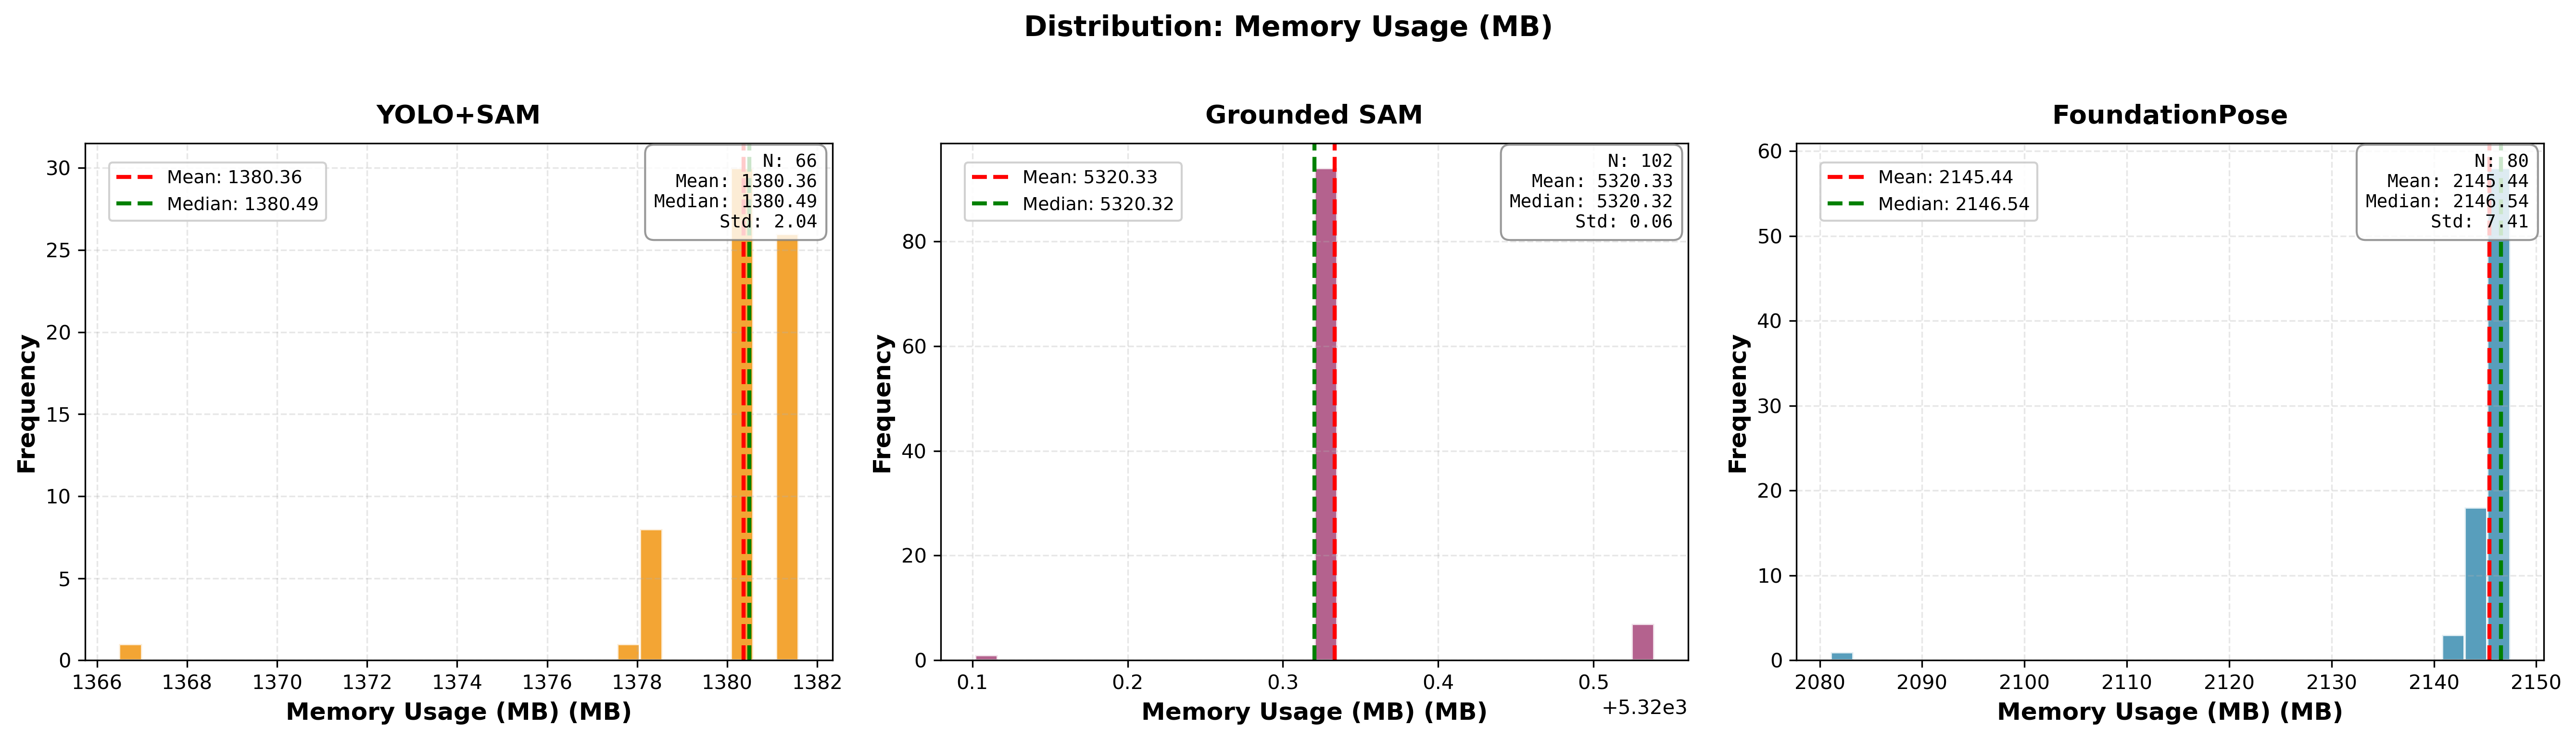
\includegraphics[width=0.9\linewidth,height=0.75\textheight,keepaspectratio]{../metrics/plots/distribution_memory_mb.png}
    \vspace{0.3em}
    \captionof{figure}{Distribution of Memory Usage (MB) across all implementations}
    % EXPLANATION: Histogram showing distribution of CPU memory usage across all implementations. FoundationPose: mean ~2145MB (2.1GB, very consistent), YOLO+SAM: mean ~1380MB (1.4GB, consistent). FoundationPose uses more memory because it loads object meshes, neural network models, and maintains circular buffers. Shows consistent memory usage across runs. Vertical lines indicate mean (red) and median (green) for each implementation.
\end{frame}

\begin{frame}
\frametitle{Performance Distribution: GPU Memory}
% EXPLANATION: This slide shows the distribution plot (histogram) for GPU memory allocation across all implementations. Provides insight into GPU memory consumption patterns.
    \centering
    \vspace{-0.5em}
    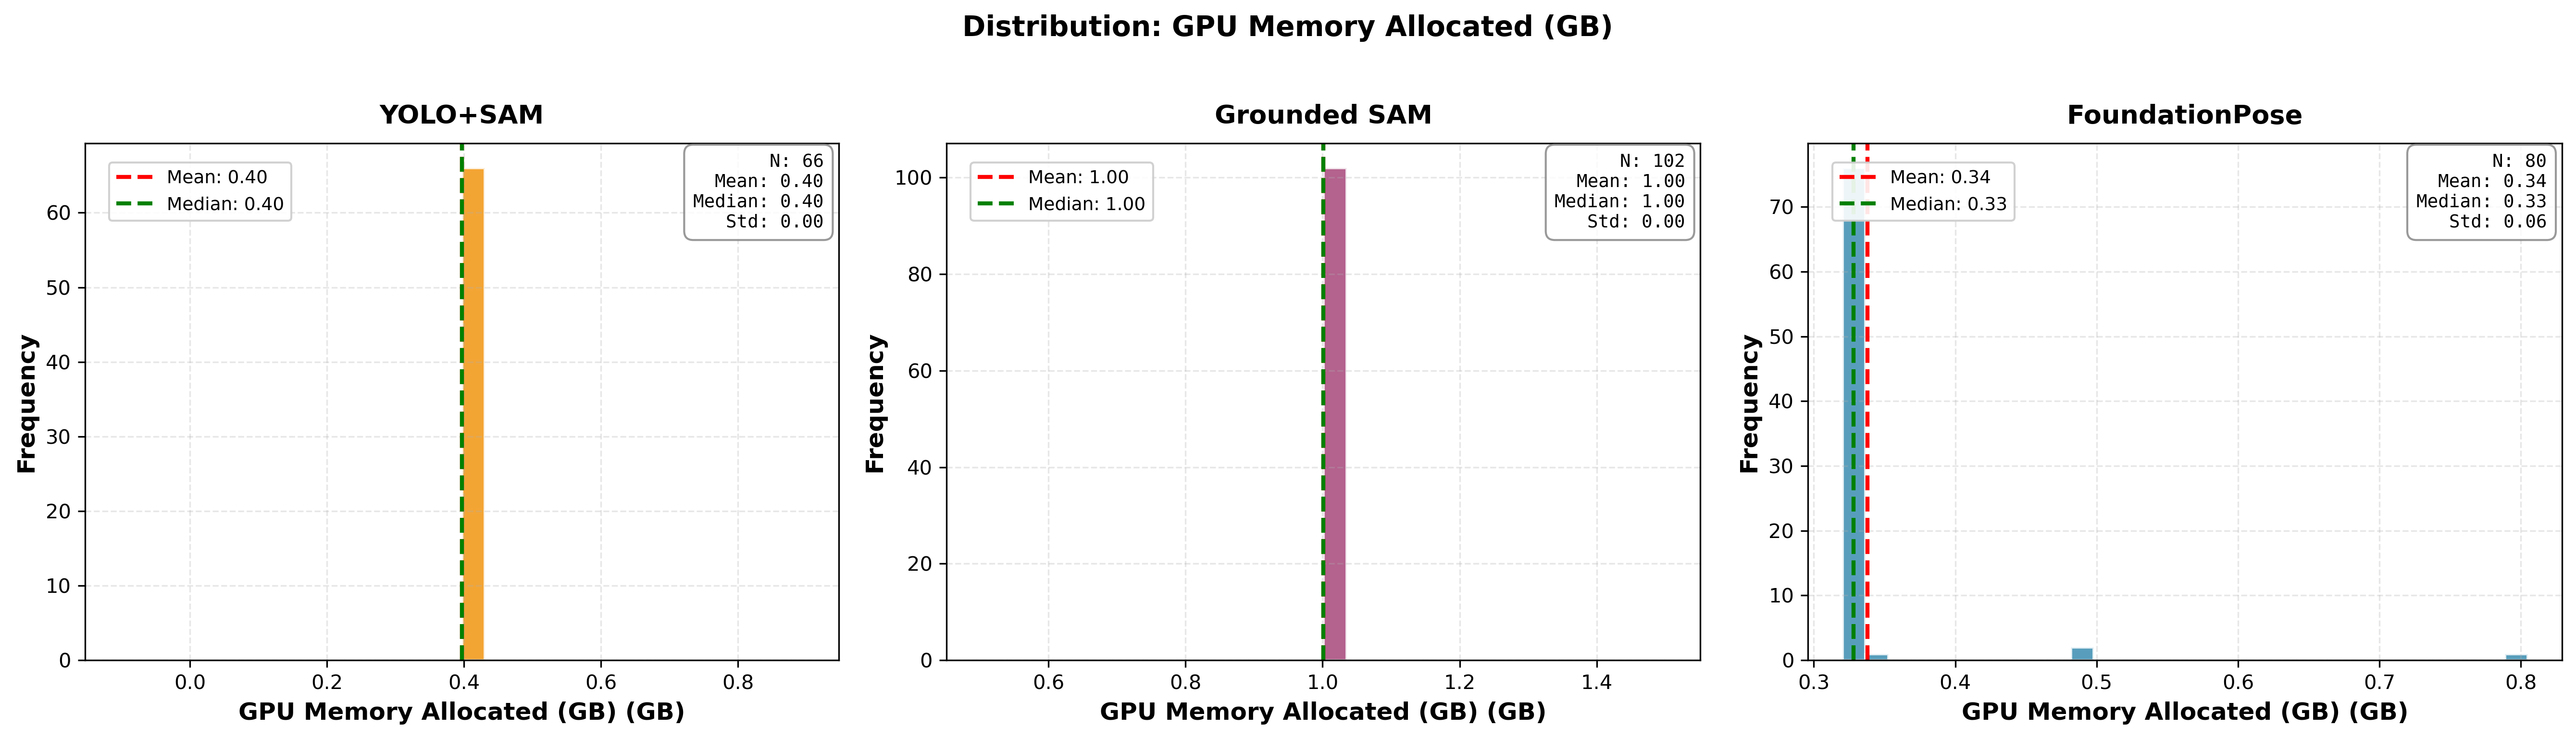
\includegraphics[width=0.9\linewidth,height=0.75\textheight,keepaspectratio]{../metrics/plots/distribution_gpu_memory_allocated_gb.png}
    \vspace{0.3em}
    \captionof{figure}{Distribution of GPU Memory Allocated (GB) across all implementations}
    % EXPLANATION: Histogram showing distribution of GPU memory allocation across all implementations. FoundationPose: mean ~0.34GB (range 0.32-0.80GB), YOLO+SAM: mean ~0.40GB (constant). FoundationPose uses GPU memory for neural network inference during dense refinement. Shows that GPU memory usage is reasonable and consistent. Vertical lines indicate mean (red) and median (green) for each implementation.
\end{frame}

\begin{frame}
\frametitle{System Evolution: Visual Comparison}
% EXPLANATION: This slide shows three video comparisons demonstrating the evolution of the system: initial implementation without segmentation (severe Z drift from depth corruption), intermediate version with segmentation but timestamp issues (drift from timestamp mismatch), and final stable system (proper segmentation + timestamp sync). Videos auto-play to show the difference.
    \centering

    \small
    \begin{minipage}{0.3\textwidth}
        \centering
        \textbf{No SAM}
        % EXPLANATION: Without segmentation mask, FoundationPose uses depth-based heuristic mask (depth between 0.3-2.0m). This includes table pixels, corrupting depth. Result: severe Z-axis (height) drift - pose jumps up and down as table pixels are included/excluded. Height error ~30cm.
    \end{minipage}
    \hfill
    \begin{minipage}{0.3\textwidth}
        \centering
        \textbf{Grounded SAM}
        % EXPLANATION: With Grounded SAM segmentation but before timestamp sync fix. Mask is clean (no table pixels), but TF lookups use wrong timestamp. Result: pose drifts over time as wrong robot poses are used. Height error ~30cm due to TF errors, not mask errors.
    \end{minipage}
    \hfill
    \begin{minipage}{0.3\textwidth}
        \centering
        \textbf{Grounded SAM + Optimized}
        % EXPLANATION: Final system with clean segmentation (Grounded SAM) and proper timestamp sync. Result: stable pose trajectory - pose updates smoothly, no drift, no jumps. Height error <2cm, position error <5cm, orientation error <10°. Suitable for manipulation.
    \end{minipage}

    \vspace{0.4em}

    \begin{minipage}{0.3\textwidth}
        \centering
        \includemedia[
            width=\linewidth,
            height=0.6\linewidth,
            activate=pageopen,
            addresource=../recordings/PoseEstimation_without_mask_fast.mp4,
            flashvars={
                source=../recordings/PoseEstimation_without_mask_fast.mp4
                &autoPlay=true
                &loop=false
                &controlBarAutoHide=true
            }
        ]{%
            \fbox{\parbox[c][2.0cm][c]{\linewidth}{\centering No mask\\(fast)}}
        }{VPlayer.swf}
        % EXPLANATION: Video shows pose estimation without segmentation mask. Pose marker (coordinate frame) jumps around, especially in Z-axis (height). This is the "severe Z drift" - height estimate is unstable because depth-based mask includes/excludes table pixels inconsistently.
    \end{minipage}
    \hfill
    \begin{minipage}{0.3\textwidth}
        \centering
        \includemedia[
            width=\linewidth,
            height=0.6\linewidth,
            activate=pageopen,
            addresource=../recordings/PoseEstimation_with_GroundedSAM_issue_fast.mp4,
            flashvars={
                source=../recordings/PoseEstimation_with_GroundedSAM_issue_fast.mp4
                &autoPlay=true
                &loop=false
                &controlBarAutoHide=true
            }
        ]{%
            \fbox{\parbox[c][2.0cm][c]{\linewidth}{\centering Grounded SAM\\issue (fast)}}
        }{VPlayer.swf}
        % EXPLANATION: Video shows pose estimation with Grounded SAM segmentation but before timestamp sync fix. Mask is clean (no table pixels), but pose still drifts over time. This is the "timestamp mismatch" issue - wrong TF transforms cause gradual drift. Demonstrates that segmentation alone isn't enough, timestamp sync is also critical.
    \end{minipage}
    \hfill
    \begin{minipage}{0.3\textwidth}
        \centering
        \includemedia[
            width=\linewidth,
            height=0.6\linewidth,
            activate=pageopen,
            addresource=../recordings/PoseEstimation_with_GroundedSAM_fast.mp4,
            flashvars={
                source=../recordings/PoseEstimation_with_GroundedSAM_fast.mp4
                &autoPlay=true
                &loop=false
                &controlBarAutoHide=true
            }
        ]{%
            \fbox{\parbox[c][2.0cm][c]{\linewidth}{\centering Grounded SAM\\final (fast)}}
        }{VPlayer.swf}
        % EXPLANATION: Video shows final stable system: Grounded SAM segmentation + timestamp sync + consensus filtering. Pose marker (coordinate frame) is stable - smooth updates, no drift, no jumps. This is the "stable SE(3) trajectory" - pose evolves smoothly in SE(3) space (rigid transformations). Suitable for manipulation.
    \end{minipage}

    \vspace{0.4em}
    \scriptsize
    Video playback requires Adobe Acrobat. All three clips auto-play when this slide opens.
\end{frame}

% ============================================================================
% SECTION 4: Lessons & Conclusion
% ============================================================================

\section{Lessons \& Conclusion}

\begin{frame}
\frametitle{Lessons Learned}
% EXPLANATION: This slide summarizes key lessons: technical insights (validation, timestamp preservation, parallelism, monitoring), scientific lessons (segmentation quality matters, timestamp sync essential, temporal filtering helps), and methodological insights (incremental improvement, measure first, trade-offs, real-world testing, robustness over speed).
    \begin{columns}
        \column{0.48\textwidth}
        \textbf{Technical Insights}
        \begin{itemize}
            \item Validate early, fail fast
            % EXPLANATION: Check mask quality, pose confidence, temporal consistency before processing. Reject bad inputs early to avoid wasting computation on garbage. This prevents false positives from being published and corrupting downstream manipulation.
            \item Preserve timestamps end-to-end
            % EXPLANATION: Store header.stamp from RGB image, pass it through entire pipeline (segmentation, pose estimation), use it for all TF lookups. This ensures temporal consistency - all data corresponds to same robot pose. Critical for accuracy.
            \item Design for parallelism
            % EXPLANATION: Use ThreadPoolExecutor to process multiple frames concurrently. Pose estimation is CPU/GPU bound (2-5s), so parallelism improves throughput without affecting latency. Enables processing backlog during slow periods.
            \item Monitor performance continuously
            % EXPLANATION: Log processing times, GPU/CPU usage, memory, pose errors. This data (stored in metrics JSON files) enables identifying bottlenecks and measuring improvements. Performance monitoring is essential for optimization.
        \end{itemize}
        \vspace{0.3em}
        \textbf{Scientific Lessons}
        \begin{itemize}
            \item Segmentation quality $\to$ pose stability
            % EXPLANATION: Core insight: bad segmentation (leaky masks) corrupts depth, causing pose instability. Good segmentation (clean masks) enables accurate depth, leading to stable poses. Segmentation is not optional - it's fundamental to accuracy.
            \item Timestamp sync essential for robotics
            % EXPLANATION: Robot motion means camera pose changes continuously. TF transforms are time-dependent. Using wrong timestamp gives wrong transform, causing drift. Timestamp sync is not optional for moving robots - it's essential.
            \item Temporal filtering reduces uncertainty
            % EXPLANATION: Averaging multiple pose estimates over time reduces noise (uncertainty decreases as 1/N). Consensus filtering (circular buffer + clustering + averaging) produces smoother, more stable poses than individual estimates.
        \end{itemize}
        \column{0.5\textwidth}
        \textbf{Methodological Insights}
        \begin{itemize}
            \item Incremental improvement works
            % EXPLANATION: Started with 17s per pose, improved step-by-step: parallel processing, consensus filtering, timestamp sync. Each improvement built on previous. Incremental approach is more manageable than trying to optimize everything at once.
            \item Measure before optimizing
            % EXPLANATION: Used metrics to identify bottlenecks (pose estimation was slow, not segmentation). Measured errors to identify problems (height error from mask leakage, drift from timestamp mismatch). Data-driven optimization is more effective than guessing.
            \item Trade-offs are inevitable
            % EXPLANATION: Grounded SAM is slower (~680ms) than YOLO+SAM (~360ms) but more flexible (open vocabulary). Parallel processing improves throughput but increases memory usage. Must balance speed, accuracy, flexibility, resource usage.
            \item Real-world testing is essential
            % EXPLANATION: Simulation (IsaacSim) is good for development, but real-world testing reveals issues (timestamp sync, mask quality) that don't appear in simulation. Real-world validation is necessary before deployment.
            \item Robustness over speed
            % EXPLANATION: A fast system that fails frequently (like DOPE with 5% success rate) is worse than a slower system that works reliably. For manipulation, robustness (works consistently) is more important than raw speed (as long as latency is acceptable).
        \end{itemize}
        \vspace{0.3em}
        \begin{block}{Key Takeaway}
            10-30x speedup achieved through systematic, incremental optimizations
            % EXPLANATION: Started at 17s per pose (unacceptable), ended at 1.5-2.1s per pose (acceptable). Speedup: 8-20x improvement. This was achieved through systematic optimization (parallel processing, consensus filtering, timestamp sync) rather than ad-hoc changes. All poses use registration mode (tracking not implemented).
        \end{block}
    \end{columns}
\end{frame}

\begin{frame}
\frametitle{Conclusion}
% EXPLANATION: This slide summarizes the final system characteristics: robust (handles occlusions, novel objects, various angles), fast (real-time capable), reliable (validation eliminates false positives), flexible (open vocabulary), observable (performance monitoring). Emphasizes complete ROS1 + IsaacSim integration.
    \begin{block}{Final System Characteristics}
        \begin{itemize}
            \item \textbf{Robust}: Handles novel objects, various viewing angles
            % EXPLANATION: FoundationPose's dense refinement works with partial visibility (uses whatever pixels are visible). Open-Vocabulary detection enables novel objects without retraining. System works across viewing angles because FoundationPose handles perspective changes.
            \item \textbf{Fast}: Real-time capable (~2.2s per frame)
            % EXPLANATION: Total latency: 680ms (segmentation) + 1.5s (pose estimation) = ~2.2s per pose. This is acceptable for real-time manipulation - robot can update pose fast enough for closed-loop control. All poses use registration mode (tracking not implemented).
            \item \textbf{Reliable}: Stricter validation eliminates false positives
            % EXPLANATION: Multiple validation checks (mask size, confidence thresholds, temporal consistency) reject low-quality poses before publishing. This prevents false positives from corrupting manipulation. System only publishes poses it's confident about.
            \item \textbf{Flexible}: Open-vocabulary detection supports any describable object
            % EXPLANATION: Grounded SAM enables detecting any object via text description, not limited to fixed vocabulary. This makes system adaptable to new manipulation tasks without model retraining. Just change text prompt.
            \item \textbf{Observable}: Comprehensive performance monitoring
            % EXPLANATION: System logs processing times, GPU/CPU usage, memory, pose errors to JSON files. This enables performance analysis, bottleneck identification, and continuous improvement. Metrics are essential for understanding system behavior.
        \end{itemize}
    \end{block}
    \vspace{0.3cm}
    \begin{center}
        \textbf{Pose estimation system ready for robotic manipulation}
        % EXPLANATION: System is fully integrated: ROS1 Noetic for inter-node communication, IsaacSim for realistic simulation, Docker for environment isolation. All components work together seamlessly. System estimates 6D poses suitable for robotic manipulation tasks (grasping, pick-and-place), though manipulation itself was not implemented in this project.
    \end{center}
\end{frame}

\end{document}
